\documentclass{report}
\usepackage{listings}
\usepackage{subcaption}
\usepackage{graphicx}
\usepackage{hyperref}
\graphicspath{{./images}}
\def\weight{0.7}

\title{Report on CNN/Scattering classification comparison}
\author{Alberto Carli \and Gabriele Roncolato \and Leonardo Zecchin }
\date{}

\begin{document}
\maketitle
\tableofcontents
\pagebreak

\chapter{Introduction}
This report illustrates the results of the project for the Visual Intelligence class of 2022/2023. \\
The assignment is designed to test the knowledge gained in class regarding signal analysis and wavelet theory: in particular we classified signals using \textbf{Convolutional Neural Networks} and wavelet functions, specifically the \textbf{Wavelet Scattering}. \\
In this project we implemented the code necessary to classify a given dataset first by training and testing a CNN, then by applying the Wavelet Scattering Transform and training a classifier NN with the extracted features.
Finally we compared the results obtained with these two different methods in terms of accuracy against how many epochs were used to train the classifiers. \\
For the entire project, we followed the guidelines given during the laboratory lectures.

We started using an RGB dataset but we soon switched to the grayscale version because it is considered more challenging.\\
In this study, we initially used the Convolutional Neural Network (CNN) model provided during laboratory
lectures as a baseline and compared its performance with a Neural Network (NN) model with wavelet scattering.
We then sought to improve the results of both models by experimenting with different sets of parameters, with a particular
focus on the NN and wavelet scattering parameters. \\
These are the best parameters we found for the NN models:
\begin{itemize}
  \item \textbf{Invariance scale}: $J=6$
  \item \textbf{Order of scattering}: $2$
  \item \textbf{Number of rotations}: $[8, 8]$
  \item \textbf{Quality factors}: $[2, 1]$
  \item \textbf{Learning rate}: $0.005$ 
  \item \textbf{Momentum}: $0.9$
\end{itemize}
After identifying the best parameters, we directed our attention to the CNN model.\\

Our findings revealed that the dataset was relatively small, and the loss and validation
graphs suggested that the model was overfitting. To address this issue, we restructured the
CNN model by introducing BatchNorm and Dropout layers. Results were unsatisfactory, suggesting that these changes alone were insufficient.
To address the overfitting issue, we incorporated data augmentation into the training set,
which significantly improved the results. \\
Our attempts to augment the dataset using translations and rotations were initially promising,
but we found that the CNN filters were learning the black band generated by the translations.
To avoid this, we opted to stick to rotations between -45 and 45 degrees.\\
This is the final set of parameters that we found to be optimal for this dataset:
\begin{itemize}
  \item \textbf{batch\_size}: 64
  \item \textbf{test\_perc}: 0.2
  \item \textbf{num\_samples}: 500
  \item \textbf{epoch\_val}: 1
  \item \textbf{num\_k\_folds}: 3
  \item \textbf{augmentations}: 16
  \item \textbf{weight\_decay}: 0.01
  \item \textbf{optimizer}: 0
  \item \textbf{learning\_rate}: 0.005
  \item \textbf{momentum}: 0.9 
  \item \textbf{num\_epochs}: 200
\end{itemize}


\chapter{Objectives}
The goal of this project is to explore the use of scattering transforms to improve the performance of classification models on a given dataset.\\
Specifically, we aimed to compare the performance of a CNN trained on the original dataset to a NN trained on the scattering transform of the data.\\

We then visualized the filters built by the CNN and compared them to the ones built by the scattering transform to gain some insight into what types of features each model extracted.
By accomplishing these goals we have gained a better understanding of how a CNN can iteratively learn which features are more meaningful.

\chapter{Dataset}
We used a dataset consisting of 128$\times$128 RGB images split into two categories: dogs and flowers. There are 1600 pictures of dogs and 1387 pictures of flowers.
In order to make the task less trivial we converted all samples to grayscale.

\begin{figure}[h!]
  \centering
  \begin{subfigure}[t]{0.19\textwidth}
    \centering
    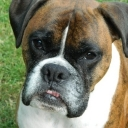
\includegraphics[width=\textwidth]{dataset/dog_0.jpg}
    \label{fig:dataset-sub1}
  \end{subfigure}
  \hfill
  \begin{subfigure}[t]{0.19\textwidth}
    \centering
    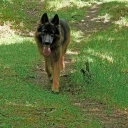
\includegraphics[width=\textwidth]{dataset/dog_1.jpg}
    \label{fig:dataset-sub2}
  \end{subfigure}
  \hfill
  \begin{subfigure}[t]{0.19\textwidth}
    \centering
    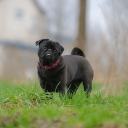
\includegraphics[width=\textwidth]{dataset/dog_2.jpg}
    \label{fig:dataset-sub3}
  \end{subfigure}
  \hfill
  \begin{subfigure}[t]{0.19\textwidth}
    \centering
    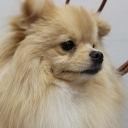
\includegraphics[width=\textwidth]{dataset/dog_3.jpg}
    \label{fig:dataset-sub4}
  \end{subfigure}
  \hfill
  \begin{subfigure}[t]{0.19\textwidth}
    \centering
    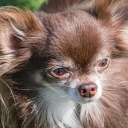
\includegraphics[width=\textwidth]{dataset/dog_4.jpg}
    \label{fig:dataset-sub5}
  \end{subfigure}

  \hfill
  \begin{subfigure}[t]{0.19\textwidth}
    \centering
    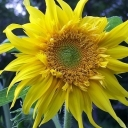
\includegraphics[width=\textwidth]{dataset/flower_0.jpg}
    \label{fig:dataset-sub1}
  \end{subfigure}
  \hfill
  \begin{subfigure}[t]{0.19\textwidth}
    \centering
    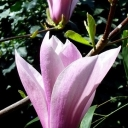
\includegraphics[width=\textwidth]{dataset/flower_1.jpg}
    \label{fig:dataset-sub2}
  \end{subfigure}
  \hfill
  \begin{subfigure}[t]{0.19\textwidth}
    \centering
    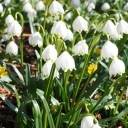
\includegraphics[width=\textwidth]{dataset/flower_2.jpg}
    \label{fig:dataset-sub3}
  \end{subfigure}
  \hfill
  \begin{subfigure}[t]{0.19\textwidth}
    \centering
    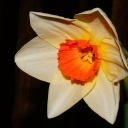
\includegraphics[width=\textwidth]{dataset/flower_3.jpg}
    \label{fig:dataset-sub4}
  \end{subfigure}
  \hfill
  \begin{subfigure}[t]{0.19\textwidth}
    \centering
    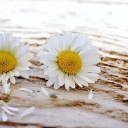
\includegraphics[width=\textwidth]{dataset/flower_4.jpg}
    \label{fig:dataset-sub5}
  \end{subfigure}

  \caption{Samples from the RGB dataset}
  \label{fig:dataset}
\end{figure}


\chapter{Framework}
\section{Convolutional Neural Network}
\subsection{What is a CNN}
A Convolutional Neural Network (\textbf{CNN}) is a class of neural networks commonly used for visual analysis. It is designed to automatically build specialized convolutional filters and extract relevant features from input images through convolution and pooling: the extracted features can then be used to compute an output through a series of fully connected layers. \\
The \texttt{CNN\_128$\times$128} architecture consists of four \textbf{convolutional} layers and three fully connected layers. The networks takes an image with \texttt{input\_channel} channels as input and returns a vector with \texttt{num\_classes} elements representing the probability of each class as output.

\subsection{Architecture}
\begin{lstlisting}[language=bash]
CNN_128x128(
    (conv1): Conv2d(1, 16, kernel_size=(7, 7), stride=(2, 2), padding=(1, 1))
    (conv2): Conv2d(16, 32, kernel_size=(5, 5), stride=(2, 2), padding=(1, 1))
    (conv3): Conv2d(32, 64, kernel_size=(3, 3), stride=(2, 2), padding=(1, 1))
    (batchnorm1): BatchNorm2d(16, eps=1e-05, momentum=0.1, affine=True, track_running_stats=True)
    (batchnorm2): BatchNorm2d(32, eps=1e-05, momentum=0.1, affine=True, track_running_stats=True)
    (batchnorm3): BatchNorm2d(64, eps=1e-05, momentum=0.1, affine=True, track_running_stats=True)
    (drop1): Dropout(p=0.2, inplace=False)
    (flat): Flatten(start_dim=1, end_dim=-1)
    (fc1): Linear(in_features=256, out_features=64, bias=True)
    (drop2): Dropout(p=0.5, inplace=False)
    (fc2): Linear(in_features=64, out_features=2, bias=True)
    )
\end{lstlisting}
The model is named \texttt{CNN\_128$\times$128}: it takes a 128$\times$128 image with a number of channels specified by the \texttt{input\_channel} parameter as input 
(typically 3 channels for RGB images or 1 channel for grayscale images). The number of output classes is specified by the \texttt{num\_classes} parameter.\\
The CNN consists of three \textbf{convolutional layers} with an increasing number of output channels (16, 32, and 64, respectively). Each convolutional layer is followed by a \textbf{batch normalization layer},
a \textbf{ReLU} activation function and a \textbf{max pooling layer} with a kernel size of 2 and a stride of 2. \\
The output of the final convolutional layer is flattened and passed through two \textbf{fully connected} (FC) layers with 64 and \texttt{num\_classes} output units, respectively.
A dropout layer is present to prevent overfitting.\\

During the forwarding, each input image is convoluted, normalized and pooled before being flattened and forwarded to the FC layers.
The output of the last FC layer is a probability distribution over the \texttt{num\_classes} output classes, which can be used to make predictions about the class of the input image.


\section{Neural Network}
\subsection{Wavelet scattering}
\subsubsection{What is a wavelet scattering}
The wavelet scattering can be used to analyze signals, such sounds or images, by decomposing them into different frequency bands and time/space scales. It applies a series of wavelet transforms to the signal and breaks it down into its constituent frequency components.\\
The key idea behind wavelet scattering is to create a representation of the signal that is invariant to translations and rotations. This allows us to extract features from the signal that are resistant to changes in scale and position.
\subsubsection{How we do it}
Initially, we tried using the Python library \textbf{Kymatio} to apply a \textbf{2D wavelet scattering}, but some limitations in the Kymatio implementation led us to implement 
our own transform in \textbf{MATLAB}, mainly because the Kymatio library didn't allow us to specify some critical \textbf{parameters}. We were then able to execute MATLAB code from \textbf{Python} using 
the \textbf{matlab.engine} library. This implementation can be found in the \texttt{scatter\_helper.py} file.\\

The purpose of the code contained in \texttt{get\_scatterNet.m} is to create a \textbf{scattering network} MATLAB object for input images using 
 \textbf{Wavelet Scattering transform}.\\
This function calls the \texttt{waveletScattering2} MATLAB function from the Deep Learning Toolbox: WaveletScattering2 computes the scattering coefficients for a given image using a wavelet transform, which is then used to construct the scattering network. \\
The input arguments of the \texttt{get\_scatterNet} function are used to configure the waveletScattering2 function. Specifically, \texttt{invariance\_scale} specifies the scale of invariance of the scattering coefficients, \texttt{quality\_factors} specifies the quality factors for the wavelet transform, \texttt{num\_rotations} specifies the number of rotations used in the wavelet transform, and \texttt{images\_size} specifies the size of the input image.\\
Finally, the function returns the computed scattering network as \textbf{sn}.\\

In addition to that, we have incorporated the \texttt{scattering.m} file which calculates the \texttt{scatter} function. This function applies the 
\textbf{Scatter Transform} to all of the images which are passed as the input argument \texttt{images} using the Matlab function \texttt{scatteringTransform}. \\
The \texttt{scatteringTransform} function computes the scattering transform of the input images using the scattering network 
(\texttt{sn}).\\

Finally, we reshaped the extracted features in order to keep only the highest-order scattering coefficients after finding that our initial attempt 
to take the mean of the scattering coefficients over the spatial dimensions did not yield interesting results. We also found that keeping 
all of the coefficients gave worse results.


\subsection{Architecture}
\begin{lstlisting}[language=bash]
    NN_128x128(
      (flat): Flatten(start_dim=1, end_dim=-1)
      (fc1): Linear(in_features=40960, out_features=64, bias=True)
      (drop2): Dropout(p=0.5, inplace=False)
      (fc2): Linear(in_features=64, out_features=2, bias=True)
    )
    \end{lstlisting}
This is a neural network with \textbf{fully-connected layers} designed for image classification. Unlike Convolutional Neural Networks (CNNs), 
which are commonly used for image classification, this network does not have any convolutional layer. \\
The input of this network is an image with \texttt{input\_channel} channels and a size of 128$\times$128 pixels. The image is flattened 
using the\texttt{nn.Flatten()} layer and then passed through two \textbf{fully-connected layers}. The first fully-connected layer has 64 nodes 
and the second layer (which is also the output layer) has \texttt{num\_classes} units, which correspond to the total number of classes for the classification task.\\

The \textbf{forward method} defines the forwarding of the network: the input vector passes through the first FC layer, a ReLU activation function and finally a dropout layer.

\section{Pipeline}
It is possible to specify which model to employ by calling \texttt{configurable\_classification.classify()} with the value \texttt{True} for the
\textit{cnn} and \textit{nn} parameters.\\

Each model is handled separately as specified in the architecture section.
The global pipeline involves:
\begin{enumerate}
  \item dataset preparation
  \item train-test splitting
  \item augmentation
  \item train-validation splitting (k-fold)
  \item training
  \item validation
  \item testing
\end{enumerate}

The behavior of the pipeline is controlled through the parameters specified in the \textit{parameters.yaml} file.\\
These parameters are overwritten at every execution by running the \textit{lib/scripts/make\_settings.py} script.\\
Scatter-specific parameters are also written by the same script to a different file named \textit{scatter\_parameters.yaml}.\\

The results for each execution consist of training graphs and testing measures, which are saved in the \textit{results} folder: each set of results is saved in its own specific folder, which is incrementally numbered
at each execution. A dump containing all of the parameters used is also saved in a txt file.\\
The output consists of a graph showing the training and validation loss and accuracy for every fold,
a figure containing the confusion matrices side by side and a figure showing the filters built by the CNN.
If the \textit{display} parameter is set to \texttt{True}, then these results are displayed before the execution has terminated.\\

\subsection{Dataset preparation}
We created a class which handles the dataset \texttt{data\_handler.py}: this class provides a function to load the dataset from the disk, subsample it, split it
into separate training, validation, and test sets, wrap it into a batcher class from pytorch, transfer it to the GPU and perform data augmentation on it. \\
Each random operation is seeded with 42 to ensure consistent results.\\

When the data is loaded from the disk, every class folder is read using the \texttt{cv2.imread()} function and a list of labels is then generated by assigning a number to each class. \\
Then, if the parameter \texttt{samples} is set (e.g. not None), the dataset is subsampled by randomly selecting an equal number of images from each class up to the \texttt{samples} value specified. \\
The dataset and labels are saved as class attributes and returned as a \texttt{pytorch.Tensor()}.\\

The dataset is then split into training, validation, and test sets using the \texttt{get\_data\_split()} function, which is just a wrapper for the \texttt{train\_test\_split()} function from \texttt{sklearn.model\_selection} to 
better handle the data and seed it with a constant seed (42). \\
The \texttt{test\_perc} parameter controls the split percentage between the train set and the test set. \\

Then, if the folds parameter is set to greater than 1, the training set is split and iterated through \texttt{folds} folds using the \texttt{sklearn.model\_selection.KFold()} function. \\
Otherwise, the training set is split into a training set and a validation set using the \texttt{train\_test\_split()} function from \texttt{sklearn.model\_selection} with 20\% of the dataset reserved for validation. \\
The validation set is used to monitor the training process and to detect overfitting. \\

\subsection{Augmentation}
The \texttt{data\_handler} class provides a method to perform data augmentation on the dataset. This is just a wrapper function for some \texttt{torchvision.transforms} 
linked to an augmentation policy. Aternative (or custom) policies can be found in the file \texttt{lib/scripts/custom\_augment.py}. \\

The augmentation is performed by randomly applying a series of transformations to the dataset images. Our policy consists of random rotations between -45 and +45 degrees.\\

The transformations are only applied to the training set before it is split into training and validation, while the testing set is not augmented. \\
The newly generated augmented images are added to the dataset: the amount of generated images is specified by the \texttt{augmentations} parameter.\\

\subsection{Training}
The training procedure is shared between the two models. \\
The training is performed by the \texttt{train()} function in the \texttt{lib/train\_test.py} file. \\

One out of two different optimizers can be selected using the \texttt{optimizer} parameter: \texttt{0} = \texttt{SGD} or \texttt{1} = \texttt{Adam}
SGD uses \textit{learning\_rate} and \textit{momentum}, while Adam uses only \textit{learning\_rate}. \\
\textit{Cross Entropy} is used as loss function. \\

The training is performed by iterating through the training set \texttt{epochs} times. \\
The training function expects a \texttt{torch.utils.data.DataLoader} object as training set and iterates on each batch alternating classification, loss calculation and backpropagation.\\

If a GPU is available (and detected by pytorch) each batch will be loaded onto the GPU and the training will take place there. \\
The training is monitored by printing the loss and accuracy on the training set every epoch. \\
The training accuracy and loss are stored into lists and then returned after the training is done to be used for plotting. \\

\subsection{Validation}
Validation can be enabled by setting the \texttt{epoch\_val} parameter to a positive number, or disabled entirely by giving it the \texttt{None} value.
If enabled, the validation is performed once every \texttt{epoch\_val} epochs. \\

The validation is performed by setting the model to evaluation mode and iterating the model through the validation set. \\
A loss is calculated, but no backpropagation is performed.\\
If a GPU is available (and detected by pytorch), each batch will be loaded onto the GPU and the validation will take place there. \\

The validation is monitored by printing the loss and the accuracy on the validation set each time it is executed. \\
The validation accuracy and loss are stored into lists and then returned after the training is done to be used for plotting. \\
\subsection{Testing}
Testing is performed by the \texttt{test()} function in the \texttt{lib/train\_test.py} file. \\
This function expects the dataset as a \texttt{torch.utils.data.DataLoader} object and it iterates on each batch, classifying each image and storing the results \\
in the same way as the validation but using the test set. In case of data augmentation, the testing set is NOT augmented.\\

If a GPU is available (and detected by pytorch), each batch will be loaded onto the GPU and the testing will take place there. \\

The predicted results and the real results are stored and returned after the testing is done to enable a more flexible analysis and metrics calculations.\\
In our case, the \texttt{metrics} class handles the calculation of statistics and the plotting of useful graphs.\\

\chapter{Results}
Our initial dataset consisted of the RGB images and our initial models were derived from CNN defined during the laboratory lectures.\\
Starting off from this Convolutional Neural Network we extracted the fully connected
layers and used those to define the \textbf{NN\_128$\times$128} model.\\
Eventually we converted our initial dataset to grayscale images in order to make the classification task less trivial.\\

\section{Tuning scatter}
At first we focused on the NN model and on the wavelet scattering. \\
We started by tuning the parameters of the scattering transform, which are the invariance scale $J$, the order of scattering $Q$, the number of rotations $R$, and the quality factors $Q$. \\

As mentioned above, we initially tried using kymatio to apply the scattering transform but we found that the library does not support a quality factors parameter for the 2D transform: for this reason, after some fruitless parameter tuning, 
we opted to use the \texttt{scattering2d} function from \texttt{kymatio.scattering2d} which granted us more control. \\

\section{Models tuning}
We then tried tuning the parameters of the optimizer.\\
We tried using different learning rates and momentum for the SGD optimizer, and finally found the optimal values which allowed the models to start learning.
\begin{itemize}
  \item \textbf{Learning rate}: $0.01$ 
  \item \textbf{Momentum}: $0.5$
\end{itemize}

Then we finally found some good values for the MATLAB scatter transform parameters:
\begin{itemize}
  \item \textbf{Invariance scale}: $J=6$
  \item \textbf{Order of scattering}: $2$
  \item \textbf{Number of rotations}: $[8, 8]$
\end{itemize}
Using these values the neural network reached 0.81 accuracy in testing.\\

\section{CNN}
After finding the optimal scatter parameters we finally focused on the CNN model.\\
A different architecture meant, of course, the need for different parameters which could work well with the additional convolutional layers, but the model would always overfit or underfit.
After many attempts at finding an optimal configuration we concluded that the CNN model needed to be further adjusted: the addition of Batch Normalization and Dropout layers, as well as increasing or reducing the number of layers and their size, was critical in avoiding overfitting.\\
We then concluded that the best parameters for the SGD optimizer were the following:
\begin{itemize}
  \item \textbf{Learning rate}: $0.005$ 
  \item \textbf{Momentum}: $0.9$
\end{itemize}
We also attempted to use the Adam optimizer, but SGD consistently provided better results.\\

The model was now reaching a good accuracy during testing, but the filters were not quite what we expected: instead of obtaining a set of filters which resembled some generic edge detection filters (like the ones used by the scatter transform), we were obtaining some very noisy matrices.
We also started noticing a consistent tradeoff between the quality of training/accuracy and the quality of the filters.
Eventually we came to realize that, when using a small dataset, a convolutional network can either build very generic filters, which perform poorly on a very specific and biased dataset, or very specific filters, which greatly diverge from common edge detection ones but perform well on the given dataset.


\section{Augmentation}
The results showed that the only way to obtain both a good accuracy and the expected filters is to increase the training dataset.
This was not possible however, as one of the project goals was to use a small dataset: for this reason we decided to artificially increase the amount of data using data augmentation.
This allowed us to reach both reasonable training curves and the expected filters.\\

The \texttt{autoaugment} function from \texttt{torchvision.transforms} with the IMAGENET augmentation policy gave very good results.\\
In order to understand why this was the case, we tried using only a single type of transformation at a time (rotations, solarization, translations, ...).\\
Notably, when augmentation involved only translations, the filters presented some black edges and the accuracy was not as good: we concluded that the wrong type of augmentations didn't allow the model to learn any further.\\

Finally we tried using only rotations: we could see both good edge filters and decent training curves.\\
Moreover, the model's accuracy also increased.\\
We noticed a positive correlation between the number of augmented images and the quality of the filters.\\



\section{Summary}
We now present a brief summary of the parameters used to train our models.

The following are the best parameters we found for the NN model:
\begin{itemize}
  \item \textbf{Invariance scale}: $J=6$
  \item \textbf{Order of scattering}: $2$
  \item \textbf{Number of rotations}: $[8, 8]$
  \item \textbf{Quality factors}: $[2, 1]$
  \item \textbf{Learning rate}: $0.005$ 
  \item \textbf{Momentum}: $0.9$
\end{itemize}

The following are the best parameters we found for the CNN model:
\begin{itemize}
  \item \textbf{batch\_size}: 64
  \item \textbf{test\_perc}: 0.2
  \item \textbf{num\_samples}: 500
  \item \textbf{epoch\_val}: 1
  \item \textbf{num\_k\_folds}: 3
  \item \textbf{augmentations}: 16 (number of augmented images per original image)
  \item \textbf{weight\_decay}: 0.01
  \item \textbf{optimizer}: 0 (0- SGD, 1- Adam)
  \item \textbf{learning\_rate}: 0.005 (scale for how much new weights are evaluated)
  \item \textbf{momentum}: 0.9 (scale for past experience to not be perturbed by new ones)
  \item \textbf{num\_epochs}: 200
\end{itemize}
\pagebreak
\chapter{Conclusions}

Our study has revealed several key findings regarding the impact of parameter selection and data augmentation 
techniques on the performance of Convolutional Neural Networks (CNNs) and Neural Networks (NNs). The optimal 
parameters varied between the two models, but our results suggest that rotations were the most effective 
parameter for improving performance on our particular dataset.
The addition of augmented images to the dataset not only increased the overall accuracy but also allowed the CNN model to build a set of filters which resemble generic edge detection filters, in particular those used by the scatter transform.
This led us to conclude that data augmentation not only increases the capability for generalization in the fully connected layers, but also in the filters used for the convolutional layers.
Data augmentation techniques such as rotations can indeed produce filters that 
are more generalizable to new data, as the model learns to identify more robust features that are less 
dependent on a specific input. The robustness to certain properties strictly depends on the type of augmentation used: 
for example, the use of rotations led the CNN to build filters which could work well with rotated subjects, while the use of translations led the CNN to build filters which could work with black edges (although not optimal for this classification task). 
Nonetheless, it is crucial to find the right balance between the 
number and type of augmented samples and the complexity of the model to avoid overfitting. Overall, our findings 
highlight the importance of careful parameters selection and the potential benefits of using rotations as a major data 
augmentation technique for improving the performance and generalization of CNNs and NNs.

\pagebreak

\part{Appendix}
\appendix

\begin{figure}[t!]
  \centering
  \hspace{-2cm}
  \begin{subfigure}[t]{0.49\textwidth}
    \centering
    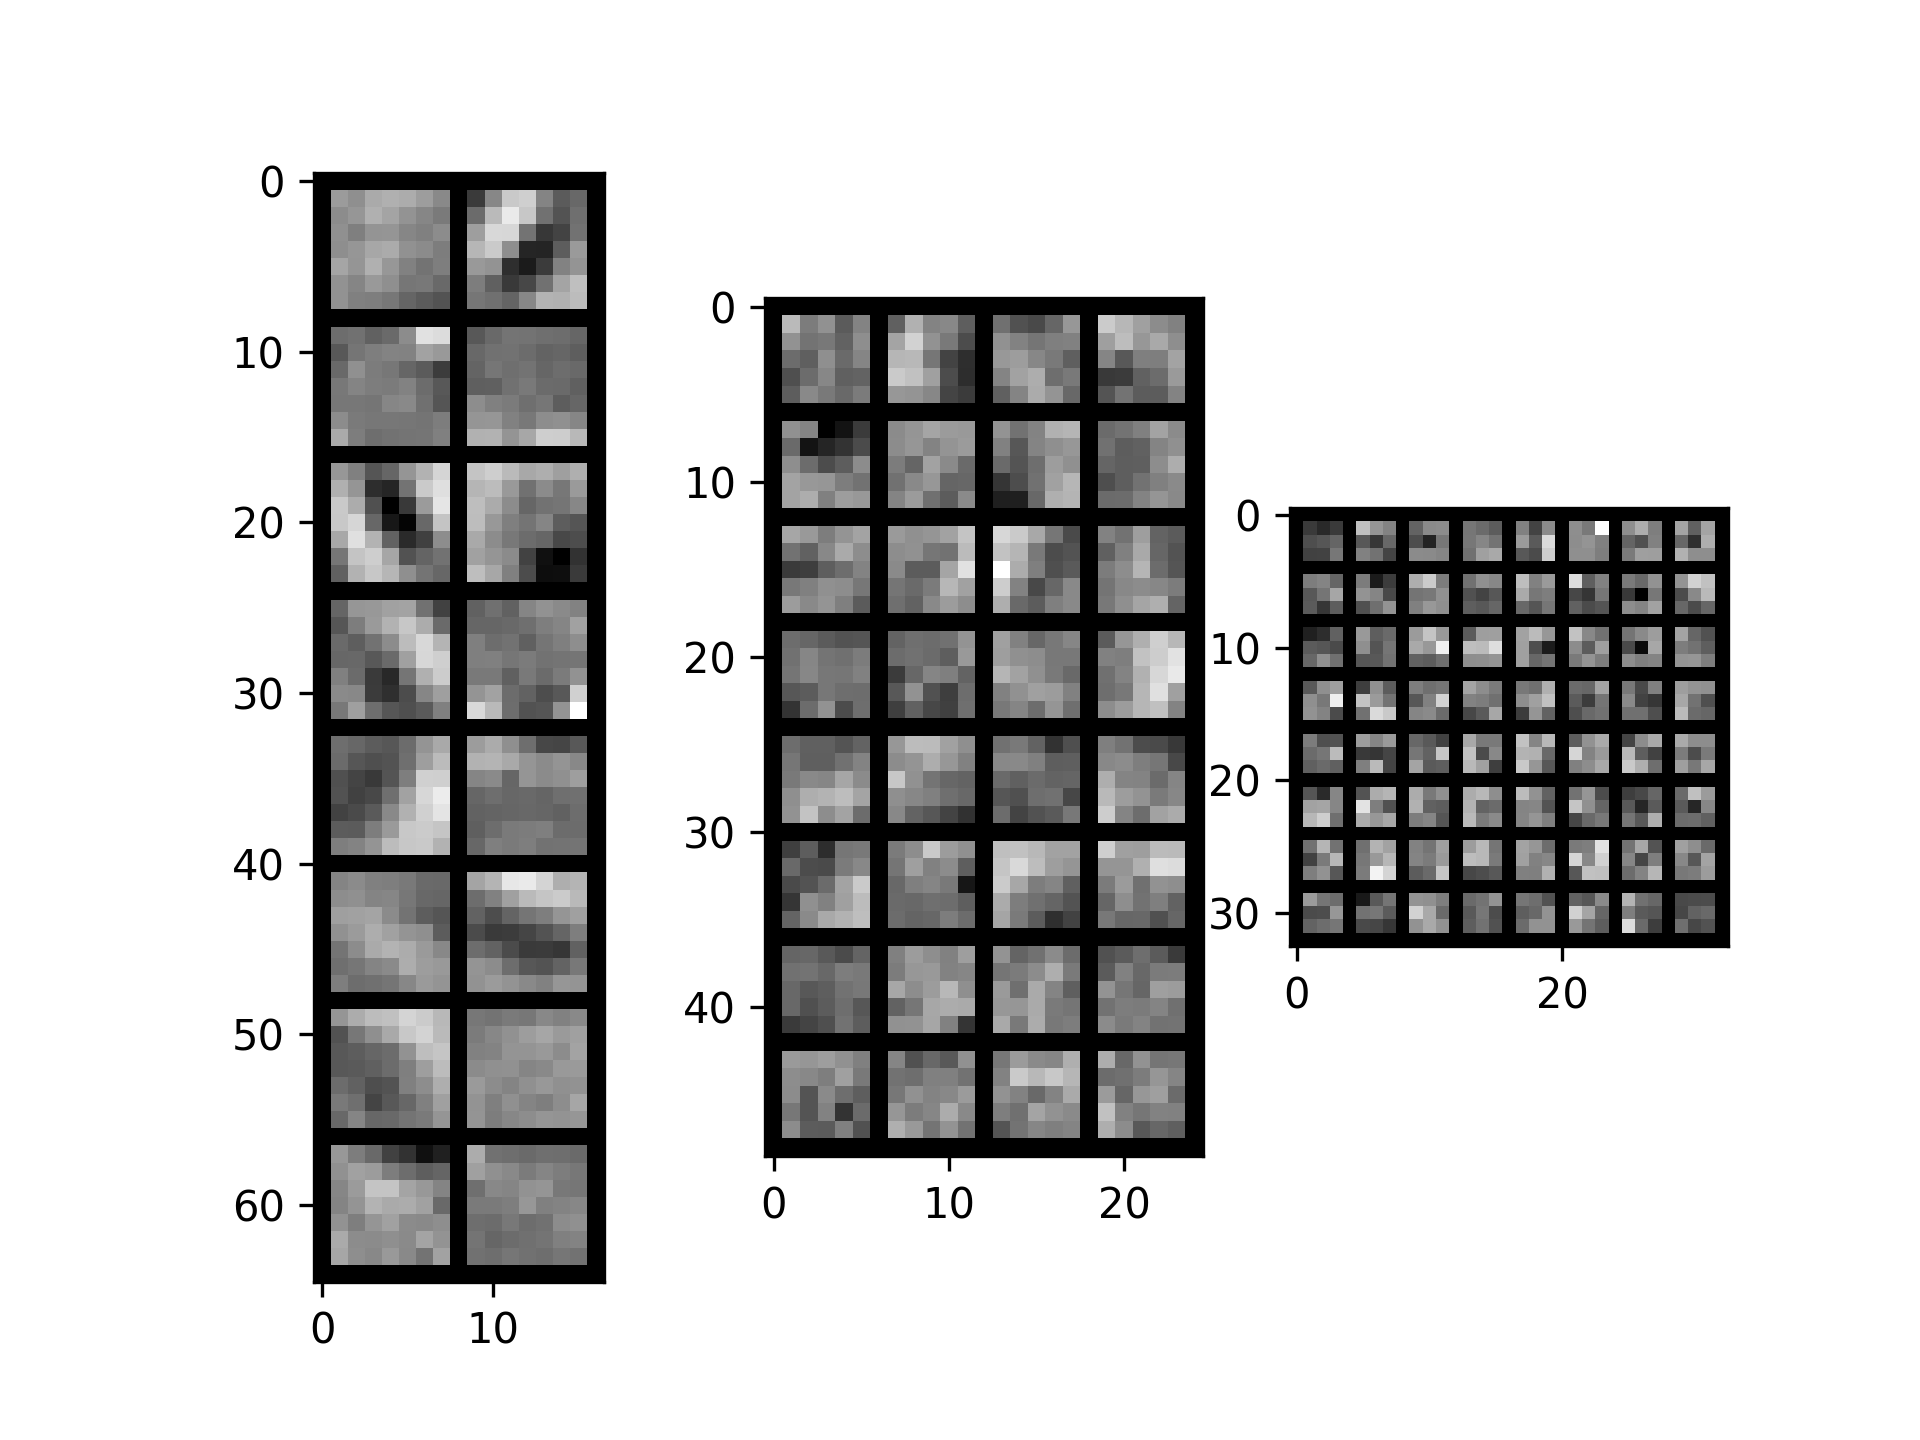
\includegraphics[width=1.3\textwidth]{3.CNN_500_sample/CNN_filters.png}
    \caption{Caption for Image 1}
    \label{fig:image-set1-sub1}
  \end{subfigure}
  \hspace{-0.5cm}
  \begin{subfigure}[t]{0.49\textwidth}
    \centering
    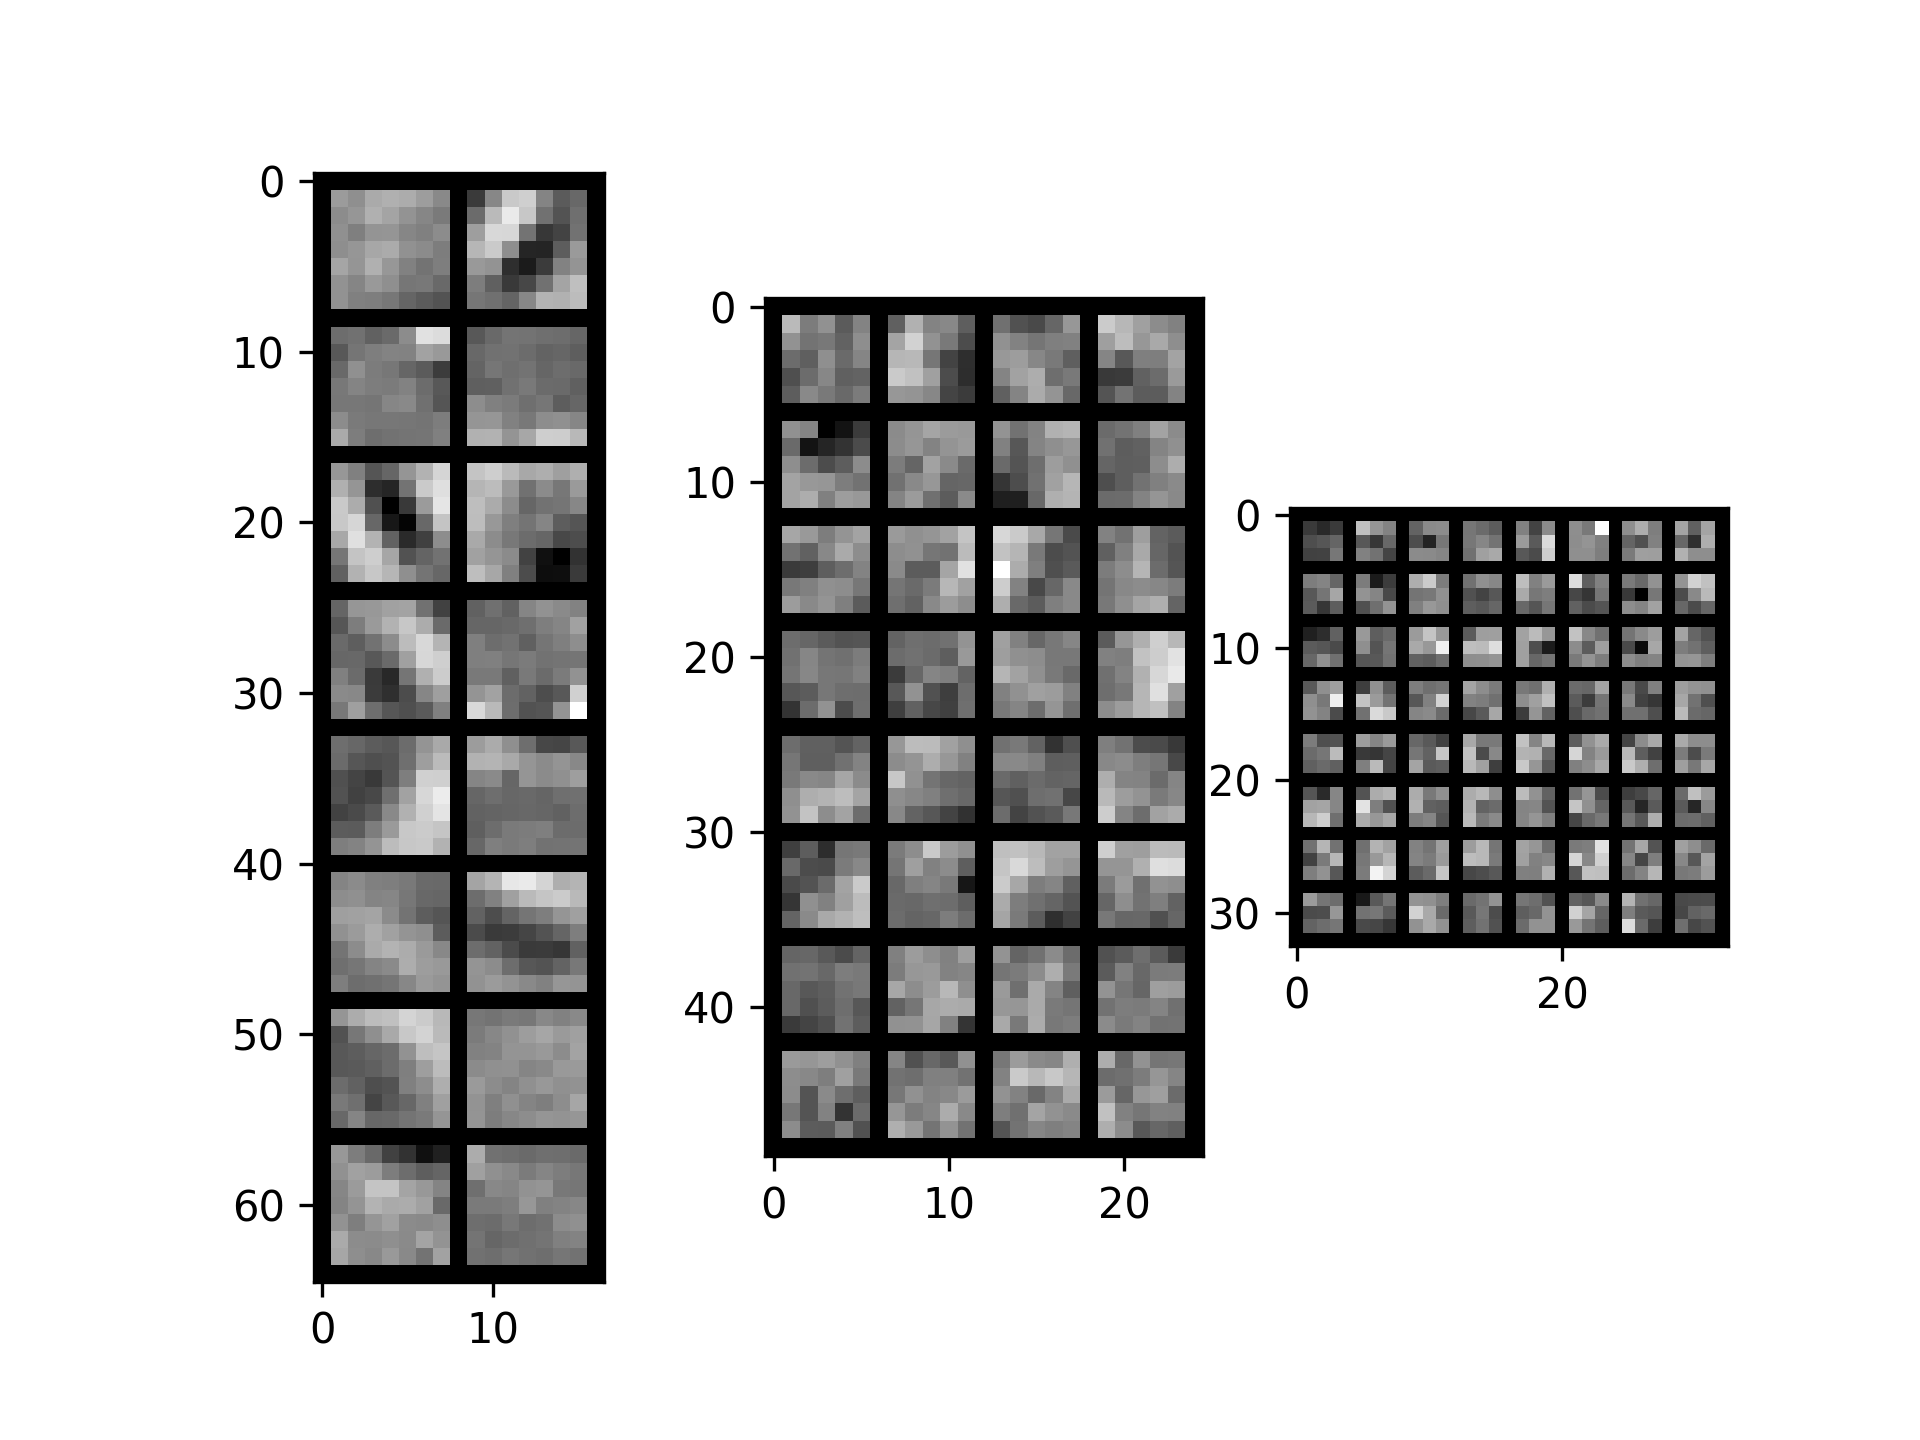
\includegraphics[width=1.3\textwidth]{3.CNN_500_sample/CNN_filters.png}
    \caption{Caption for Image 2}
    \label{fig:image-set1-sub2}
  \end{subfigure}

  \caption{Caption for the whole figure (TEMPLATE)}
  \label{fig:figure}
\end{figure}





\begin{figure}[t!]
  \centering
  \hspace{-2cm}
  \begin{subfigure}[t]{0.49\textwidth}
    \centering
    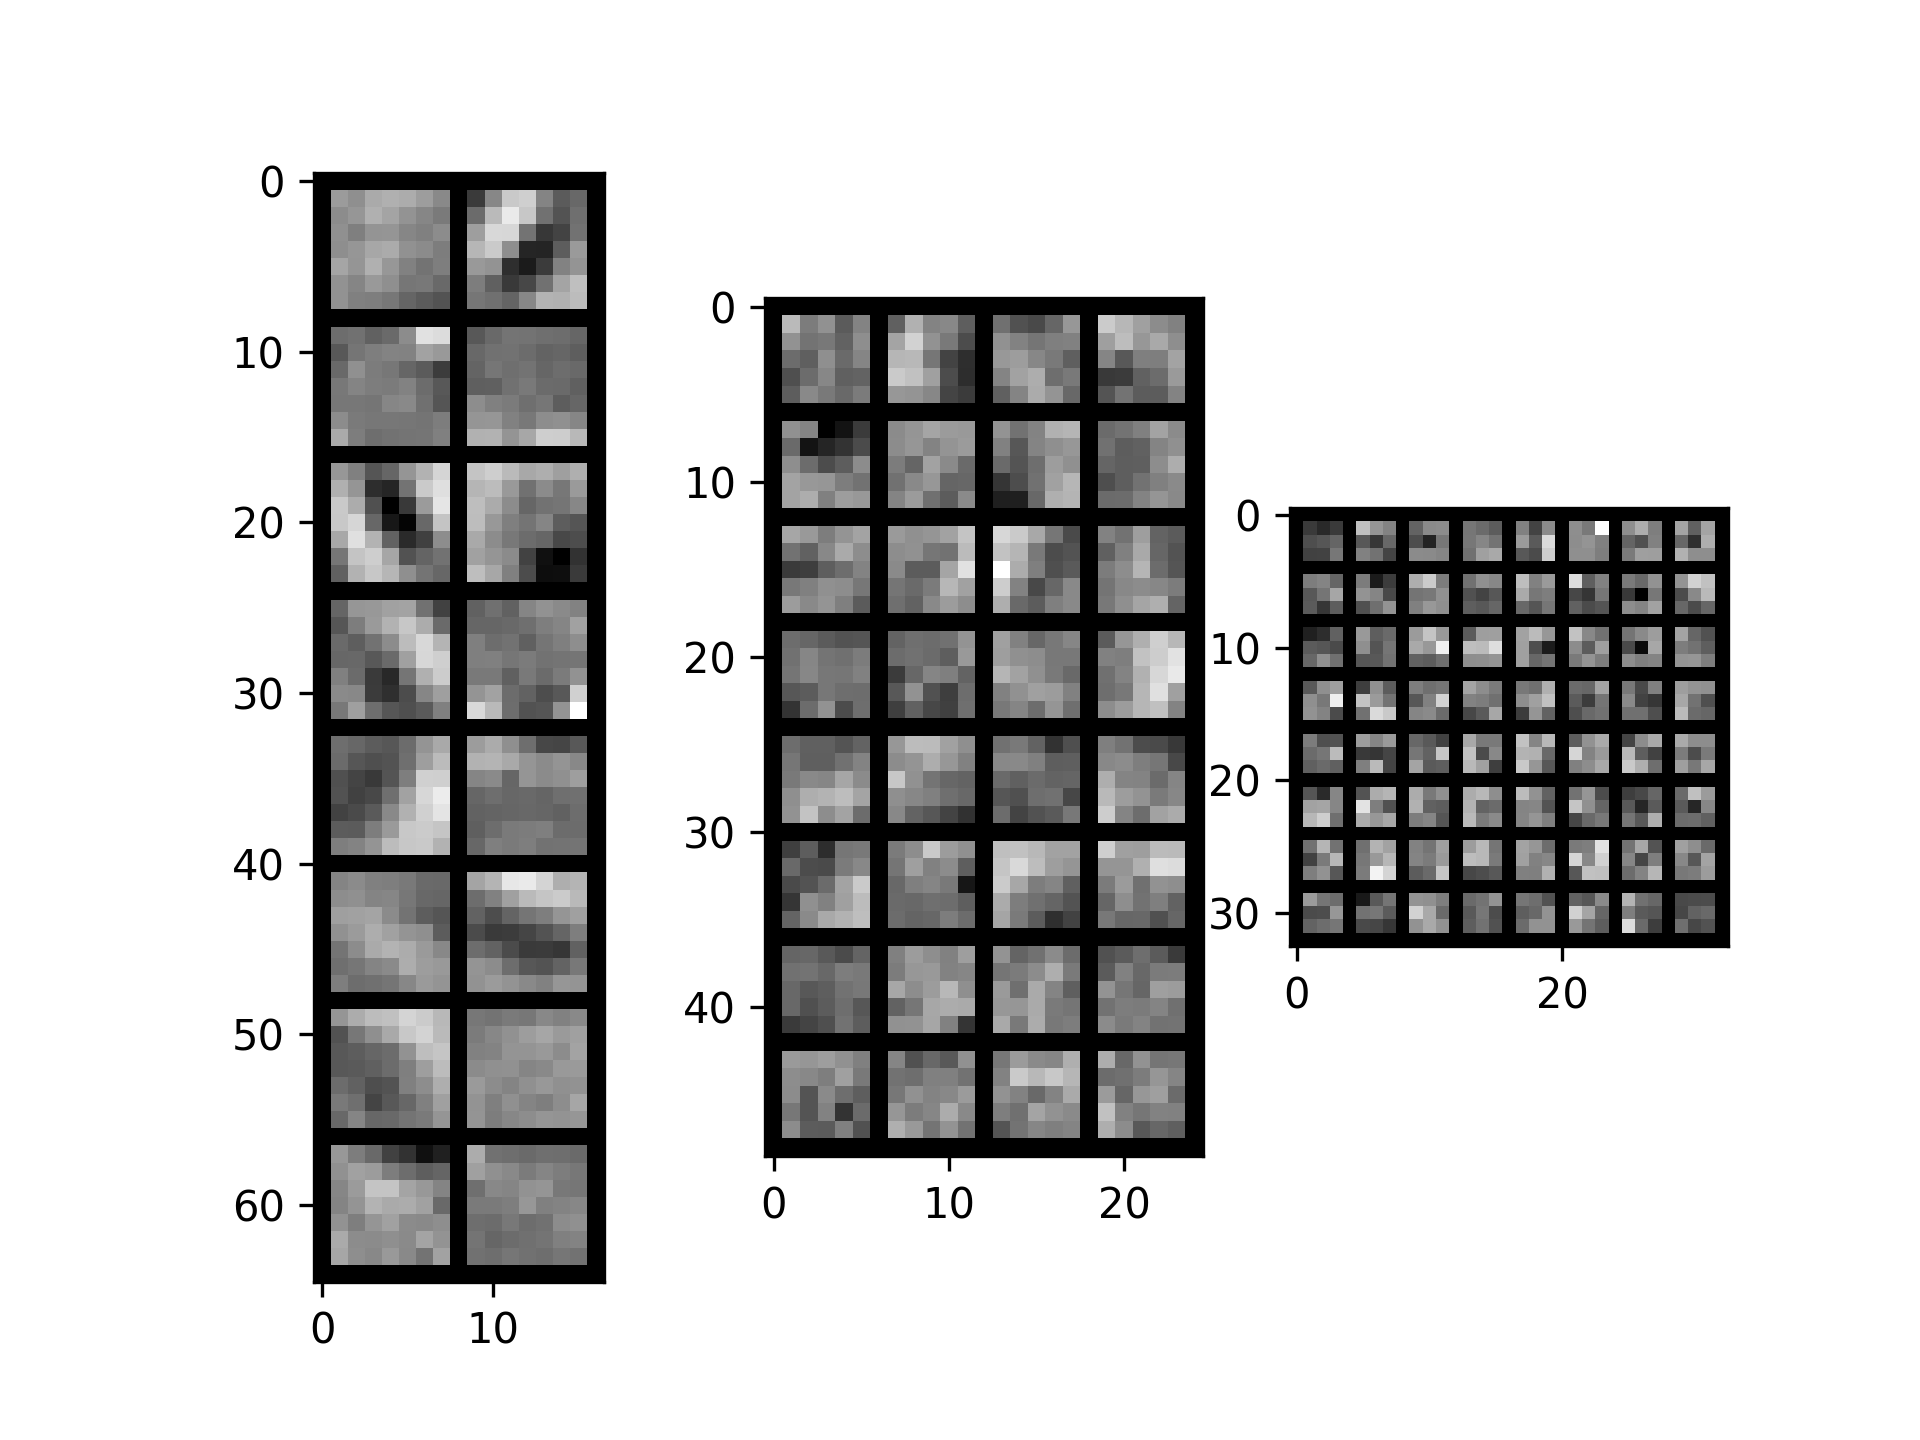
\includegraphics[width=1.3\textwidth]{3.CNN_500_sample/CNN_filters.png}
    \caption{CNN filters}
    \label{fig:image-set1-sub1}
  \end{subfigure}
  \hspace{-0.5cm}
  \begin{subfigure}[t]{0.49\textwidth}
    \centering
    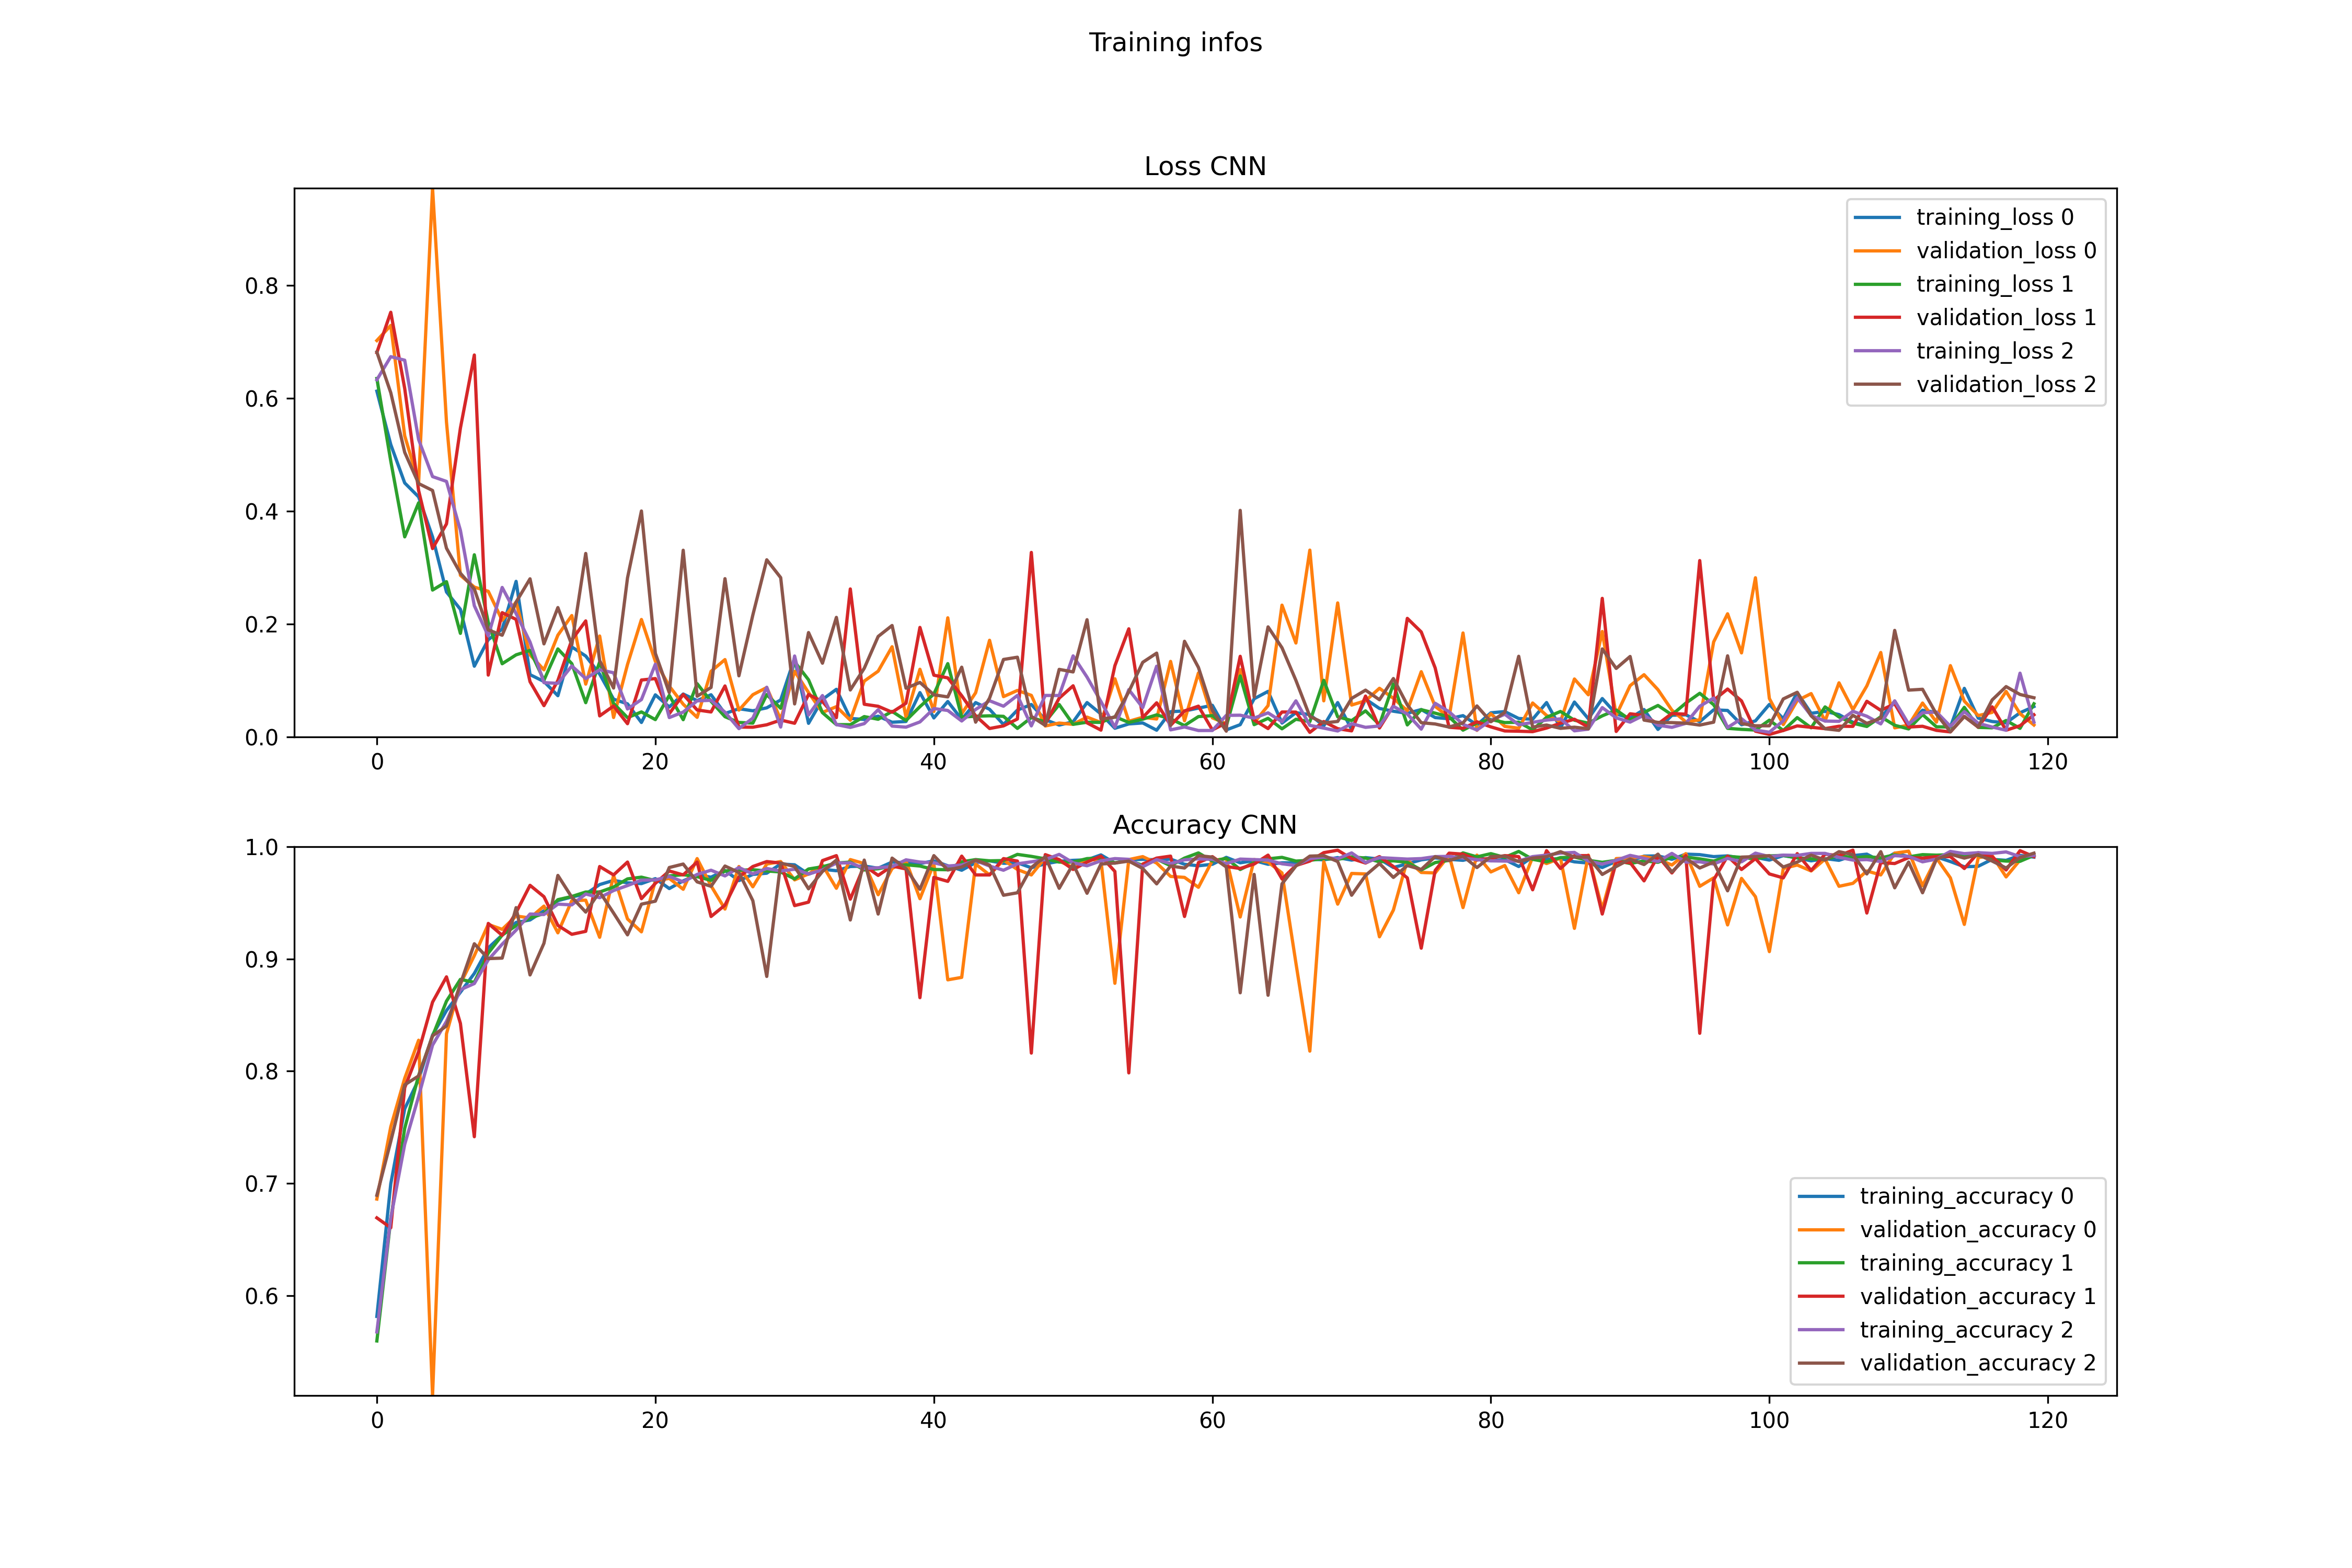
\includegraphics[width=1.3\textwidth]{3.CNN_500_sample/training_infos.png}
    \caption{Loss and Validation graphs}
    \label{fig:image-set1-sub2}
  \end{subfigure}

  \caption{These are the results obtained with the best parameters found for the CNN model. The \textbf{accuracy} reached in test is $0.82$.}
  \label{fig:image-set1}
\end{figure}

\begin{figure}[t!]
  \centering
  \hspace{-2cm}
  \begin{subfigure}[t]{0.49\textwidth}
    \centering
    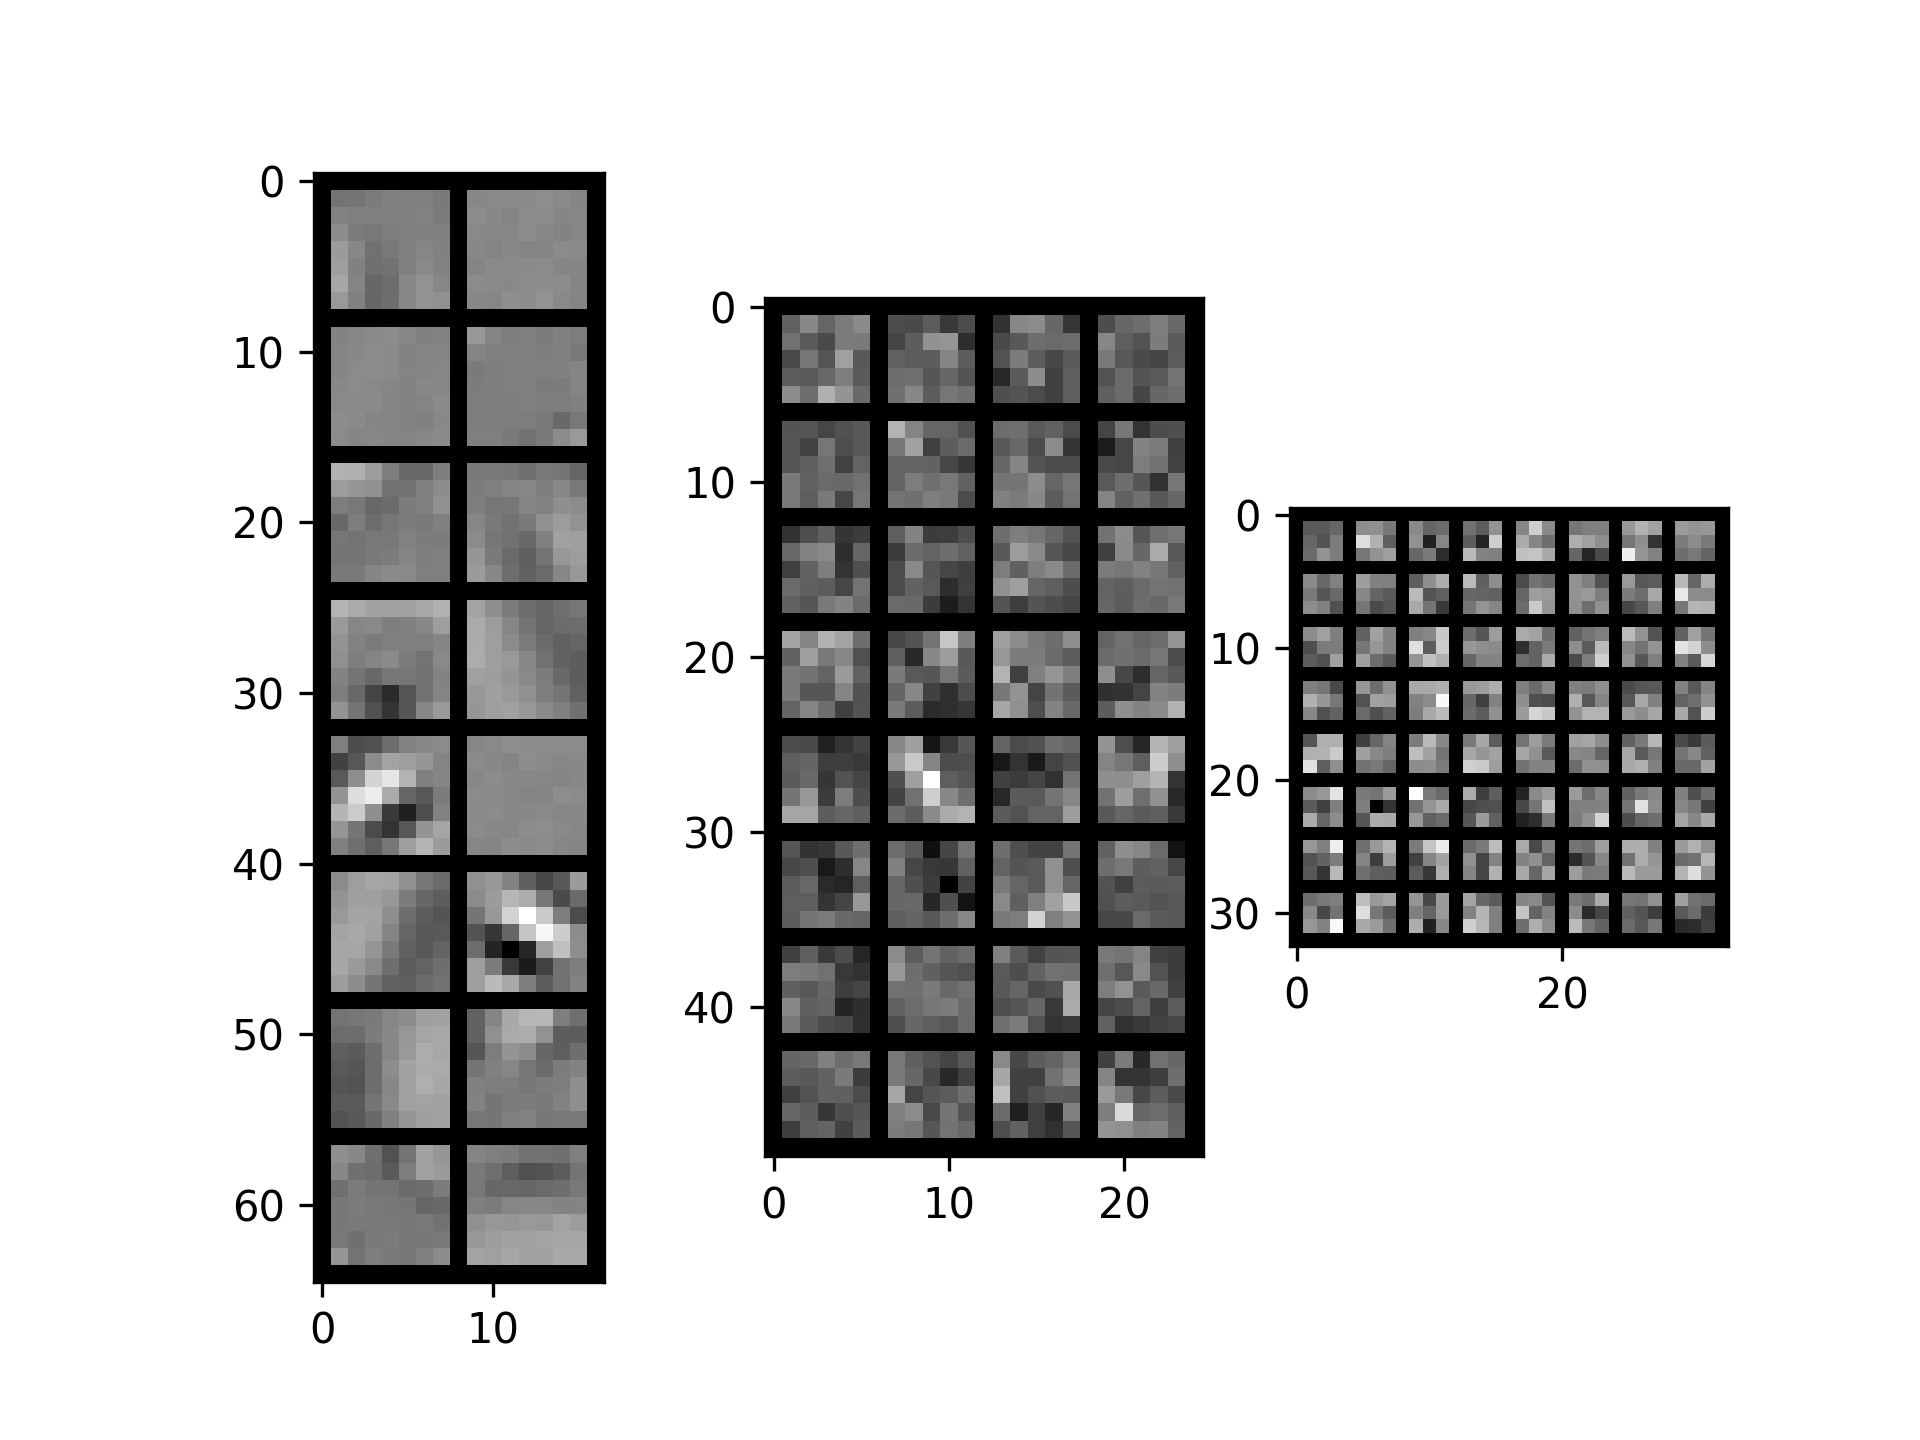
\includegraphics[width=1.3\textwidth]{4.CNN_2500_sample/CNN_filters.png}
    \caption{CNN filters}
    \label{fig:image-set2-sub1}
  \end{subfigure}
  \hspace{-0.5cm}
  \begin{subfigure}[t]{0.49\textwidth}
    \centering
    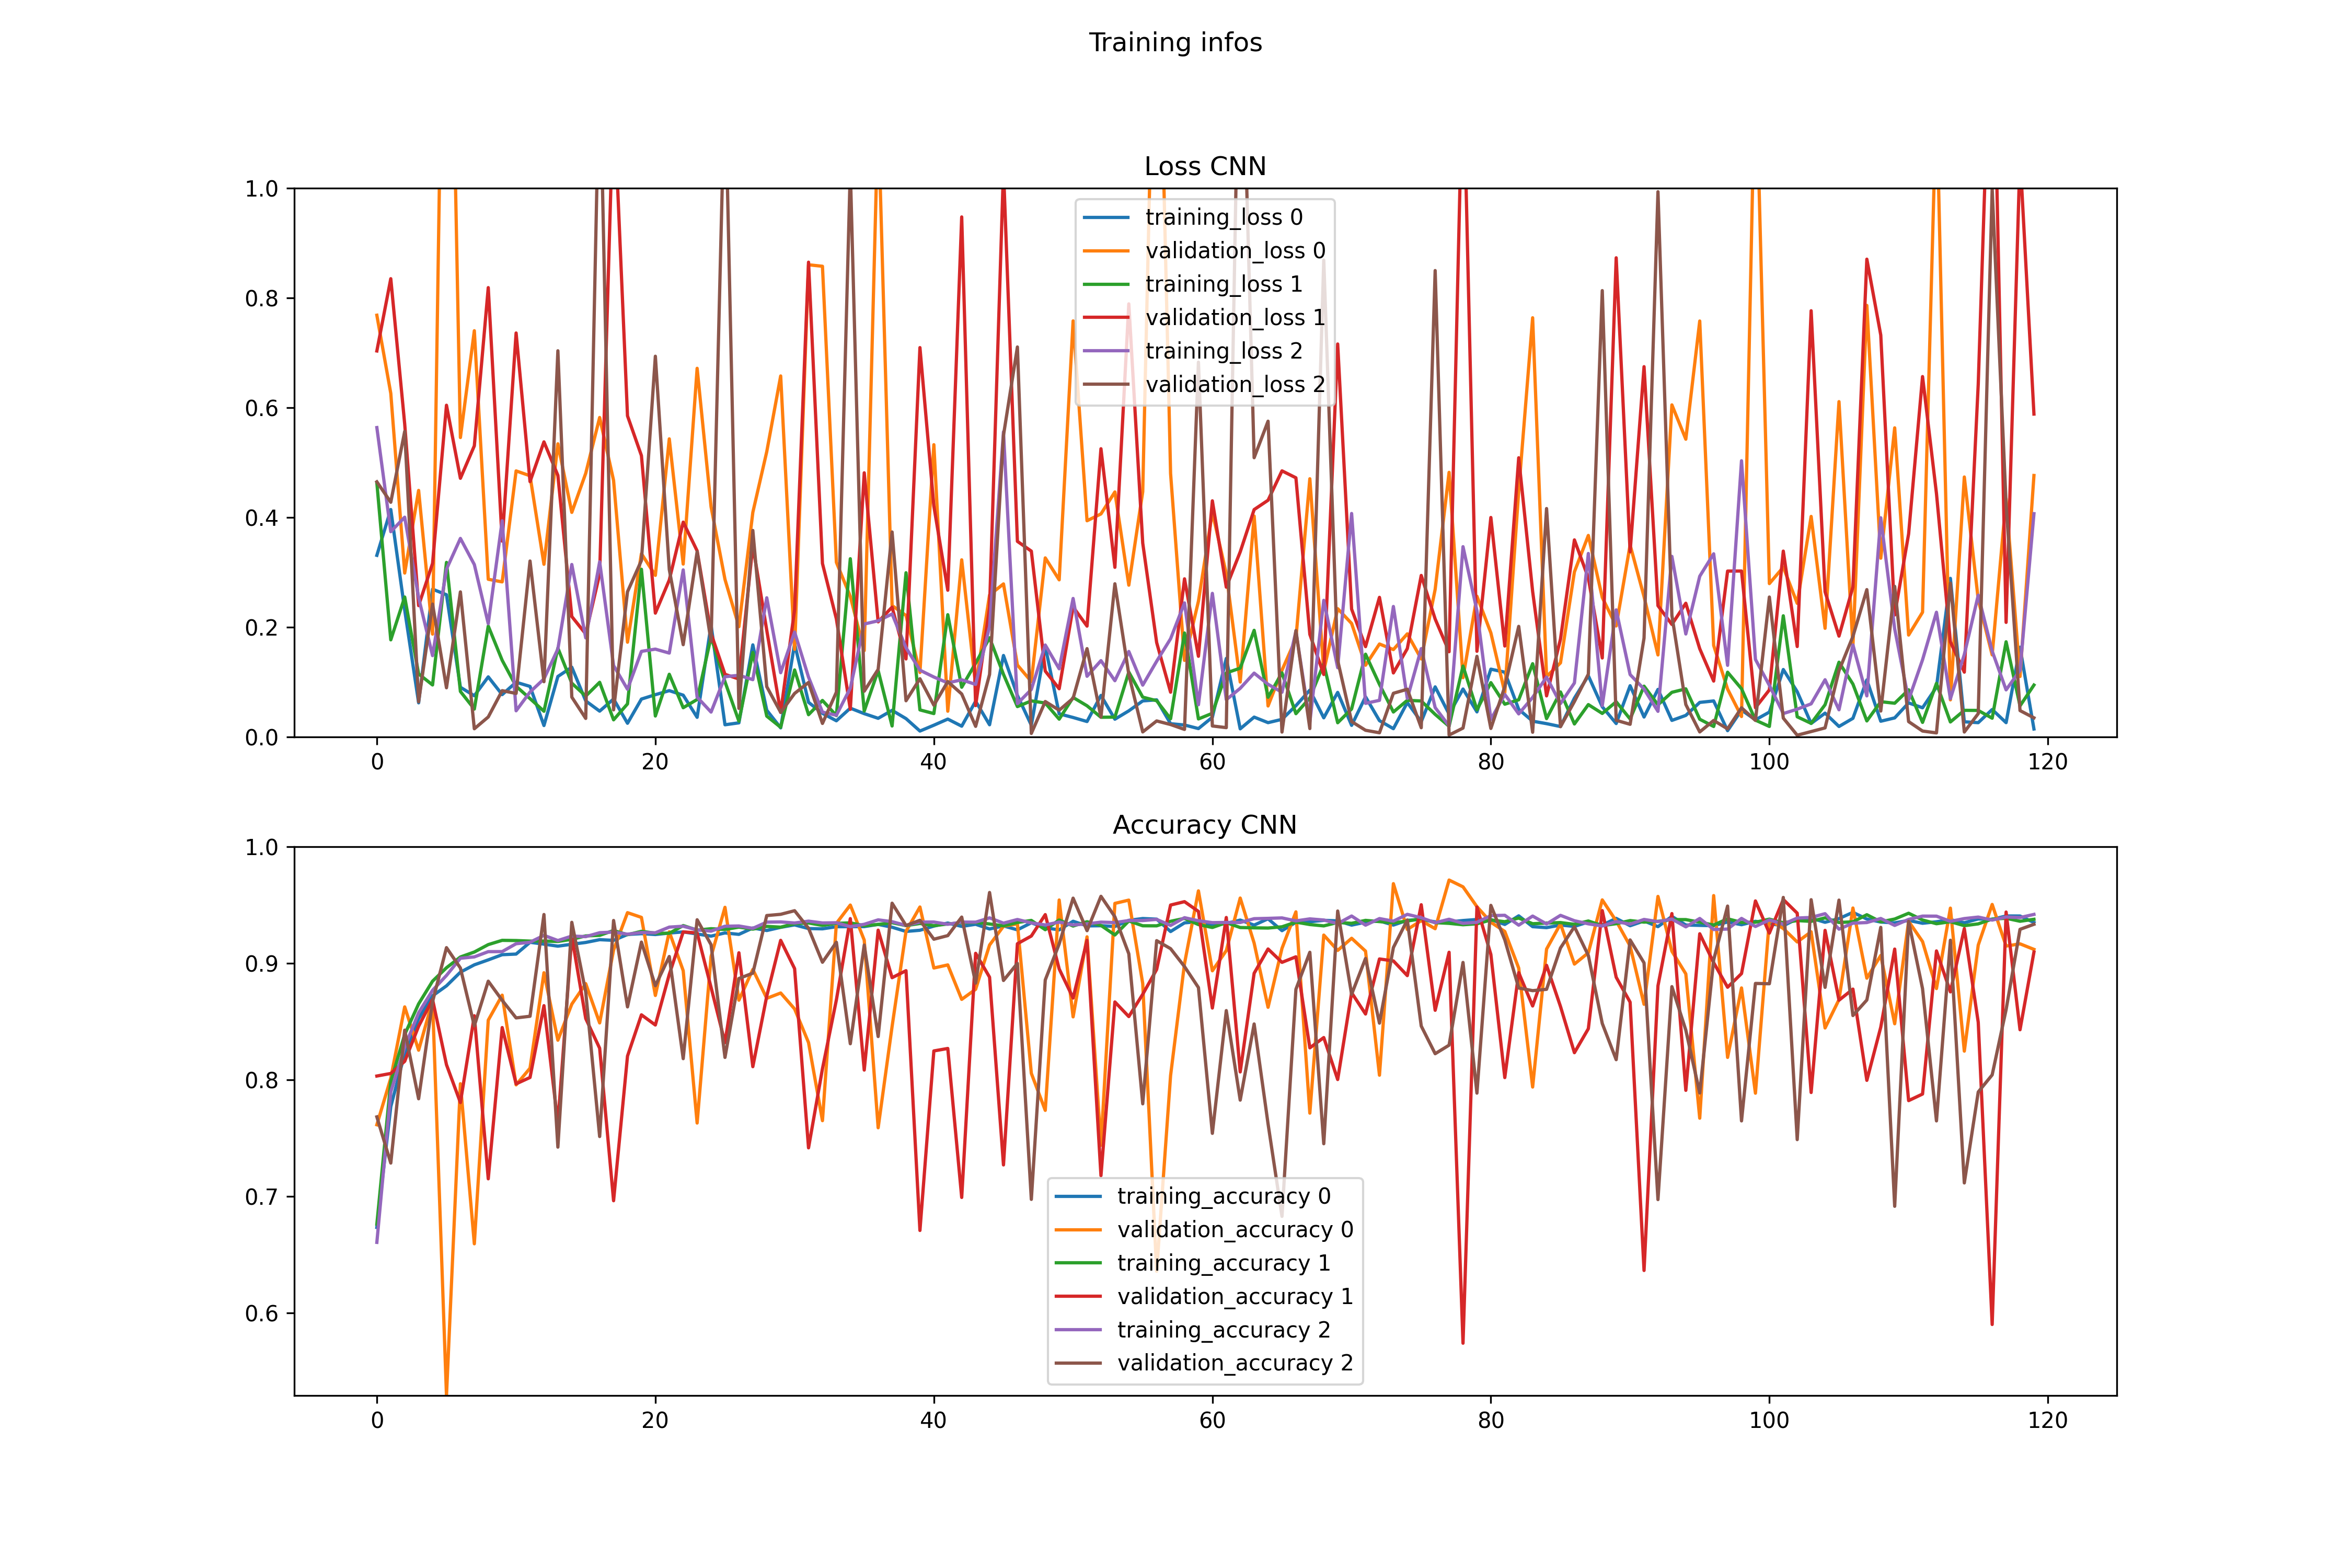
\includegraphics[width=1.3\textwidth]{4.CNN_2500_sample/training_infos.png}
    \caption{Loss and Validation graphs}
    \label{fig:image-set2-sub2}
  \end{subfigure}

  \caption{Then we tried with $2500$ samples. The \textbf{accuracy} reached in test is $0.87$
  }
  \label{fig:image-set2}
\end{figure}

\begin{figure}[t!]
  \centering
  \hspace{-2cm}
  \begin{subfigure}[t]{0.49\textwidth}
    \centering
    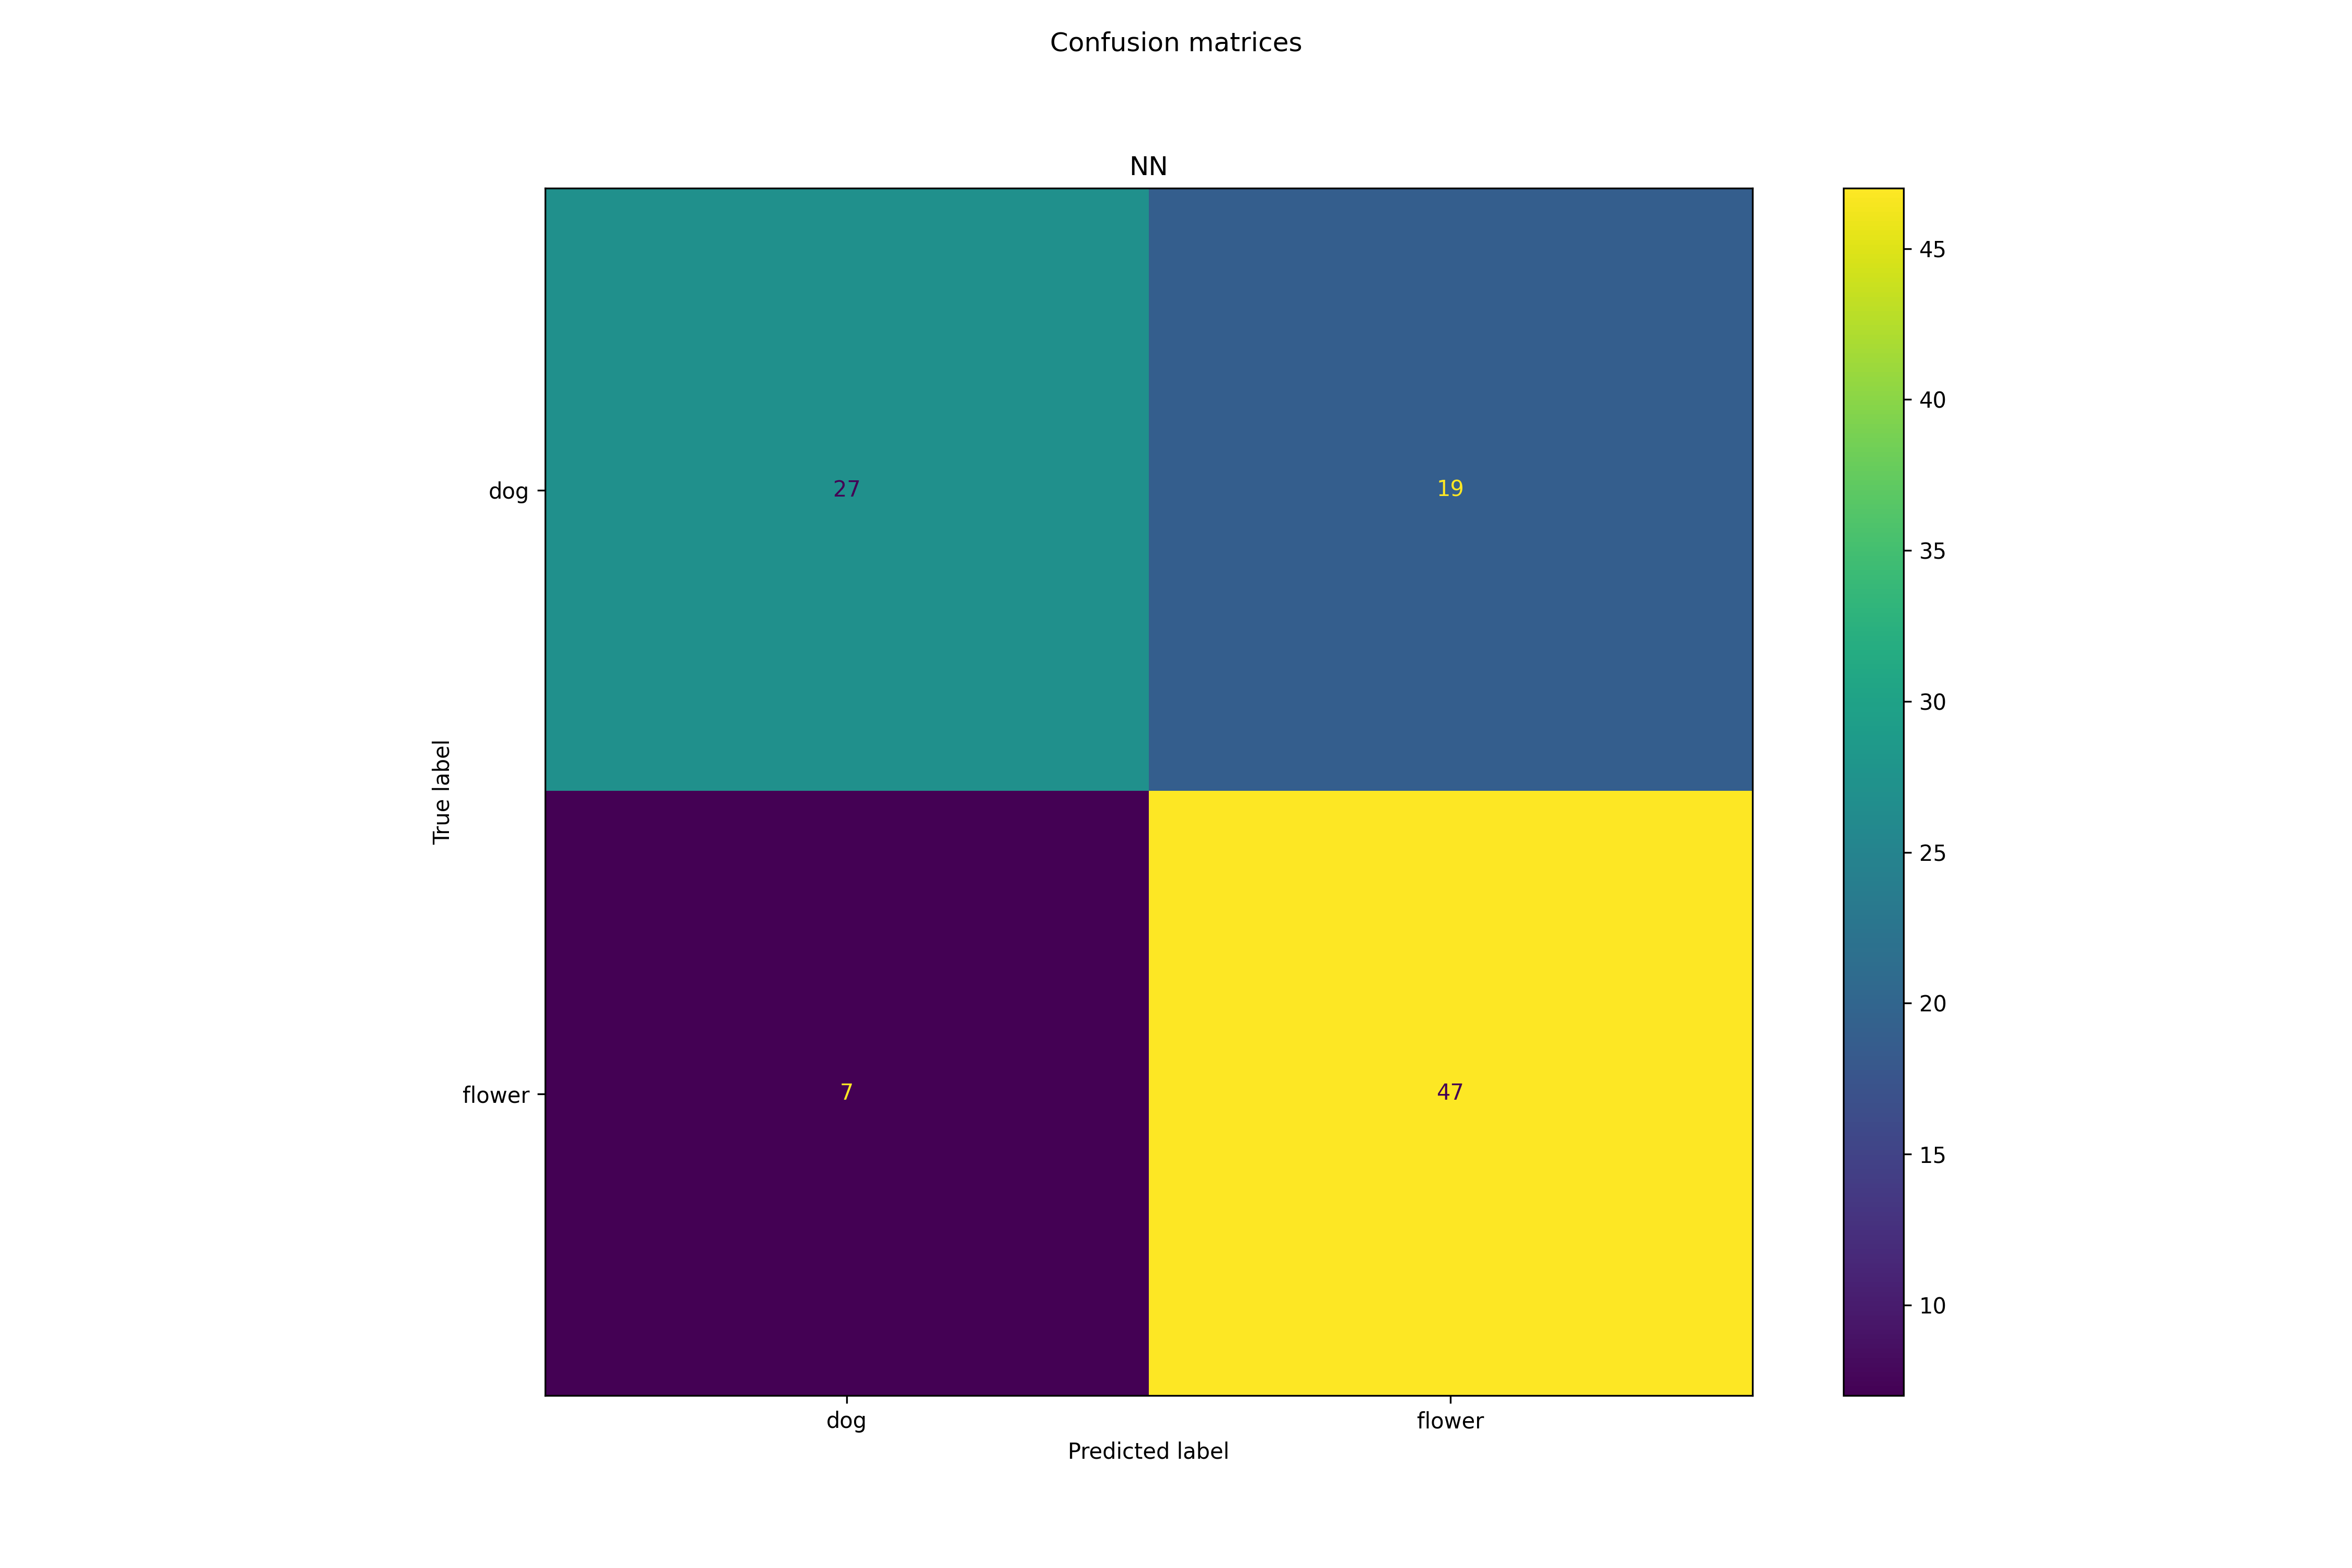
\includegraphics[width=1.3\textwidth]{1.augmentationNN/conf_mat.png}
    \caption{Confusion matrix}
    \label{fig:image-set3-sub1}
  \end{subfigure}
  \hspace{-0.5cm}
  \begin{subfigure}[t]{0.49\textwidth}
    \centering
    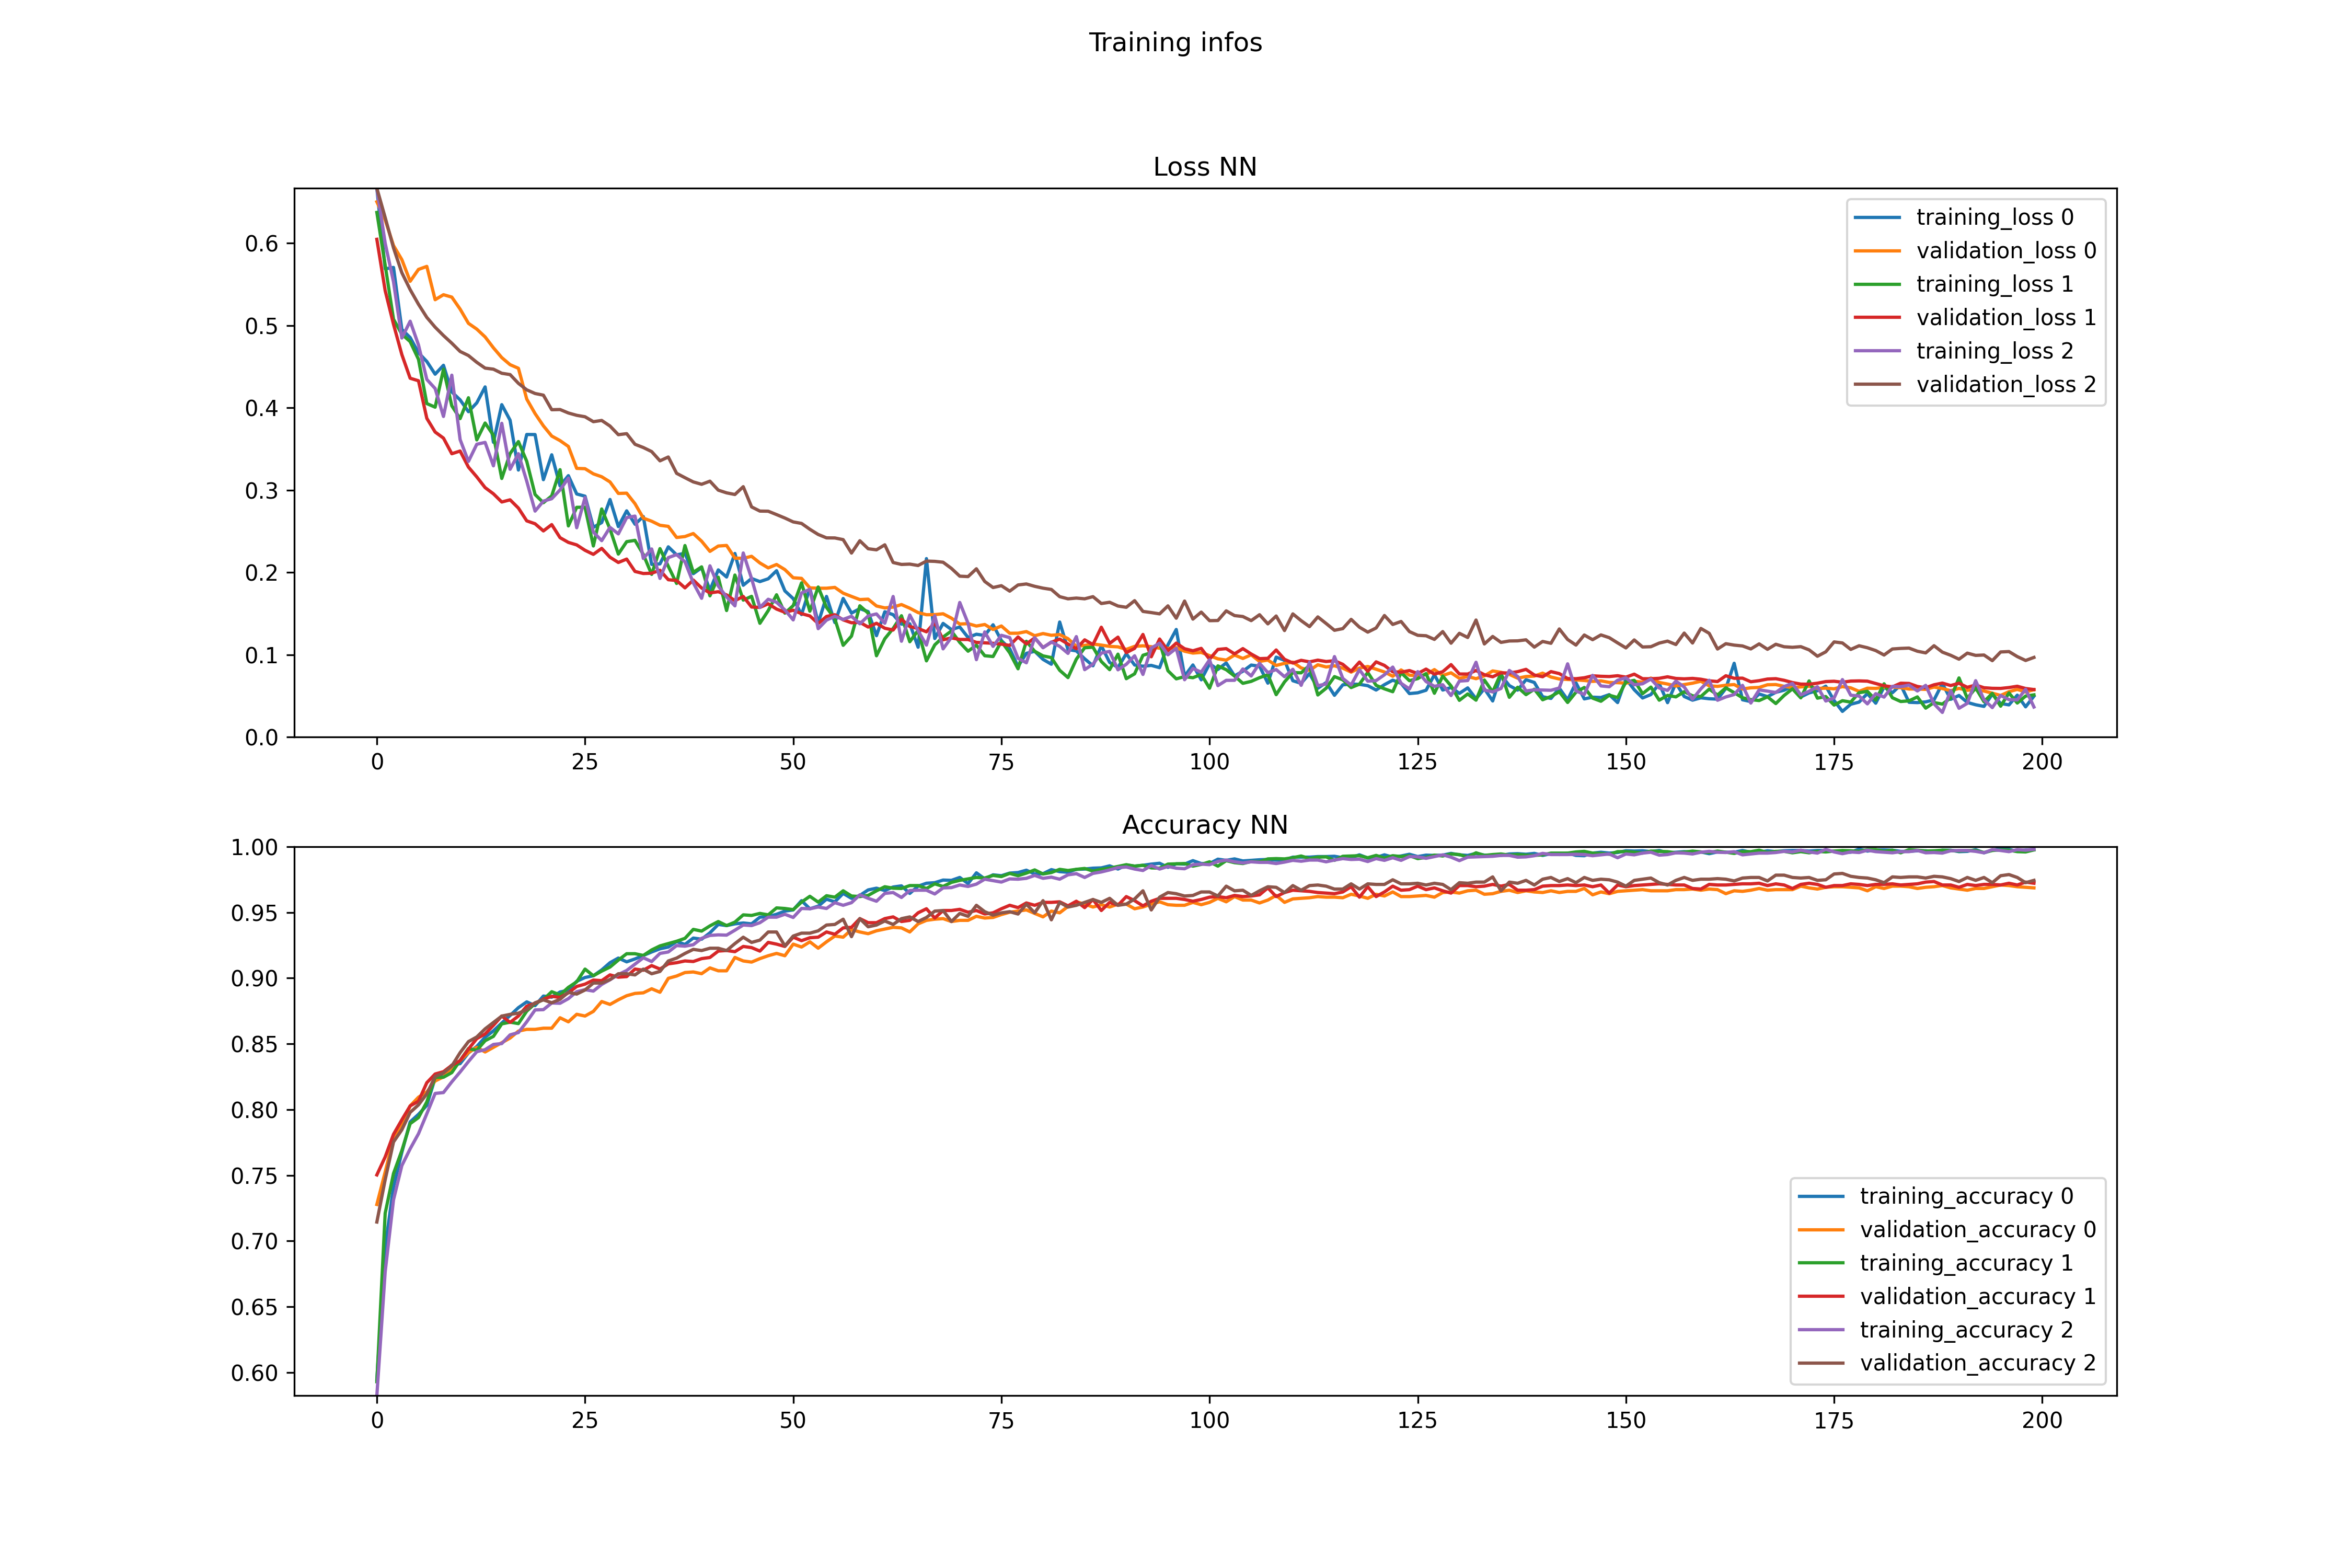
\includegraphics[width=1.3\textwidth]{1.augmentationNN/training_infos.png}
    \caption{Loss and Validation graphs}
    \label{fig:image-set3-sub2}
  \end{subfigure}

  \caption{NN executions with agumentation. The \textbf{accuracy} reached in test is $0.74$.}
  \label{fig:image-set3}
\end{figure}

\begin{figure}[t!]
  \centering
  \hspace{-2cm}
  \begin{subfigure}[t]{0.49\textwidth}
    \centering
    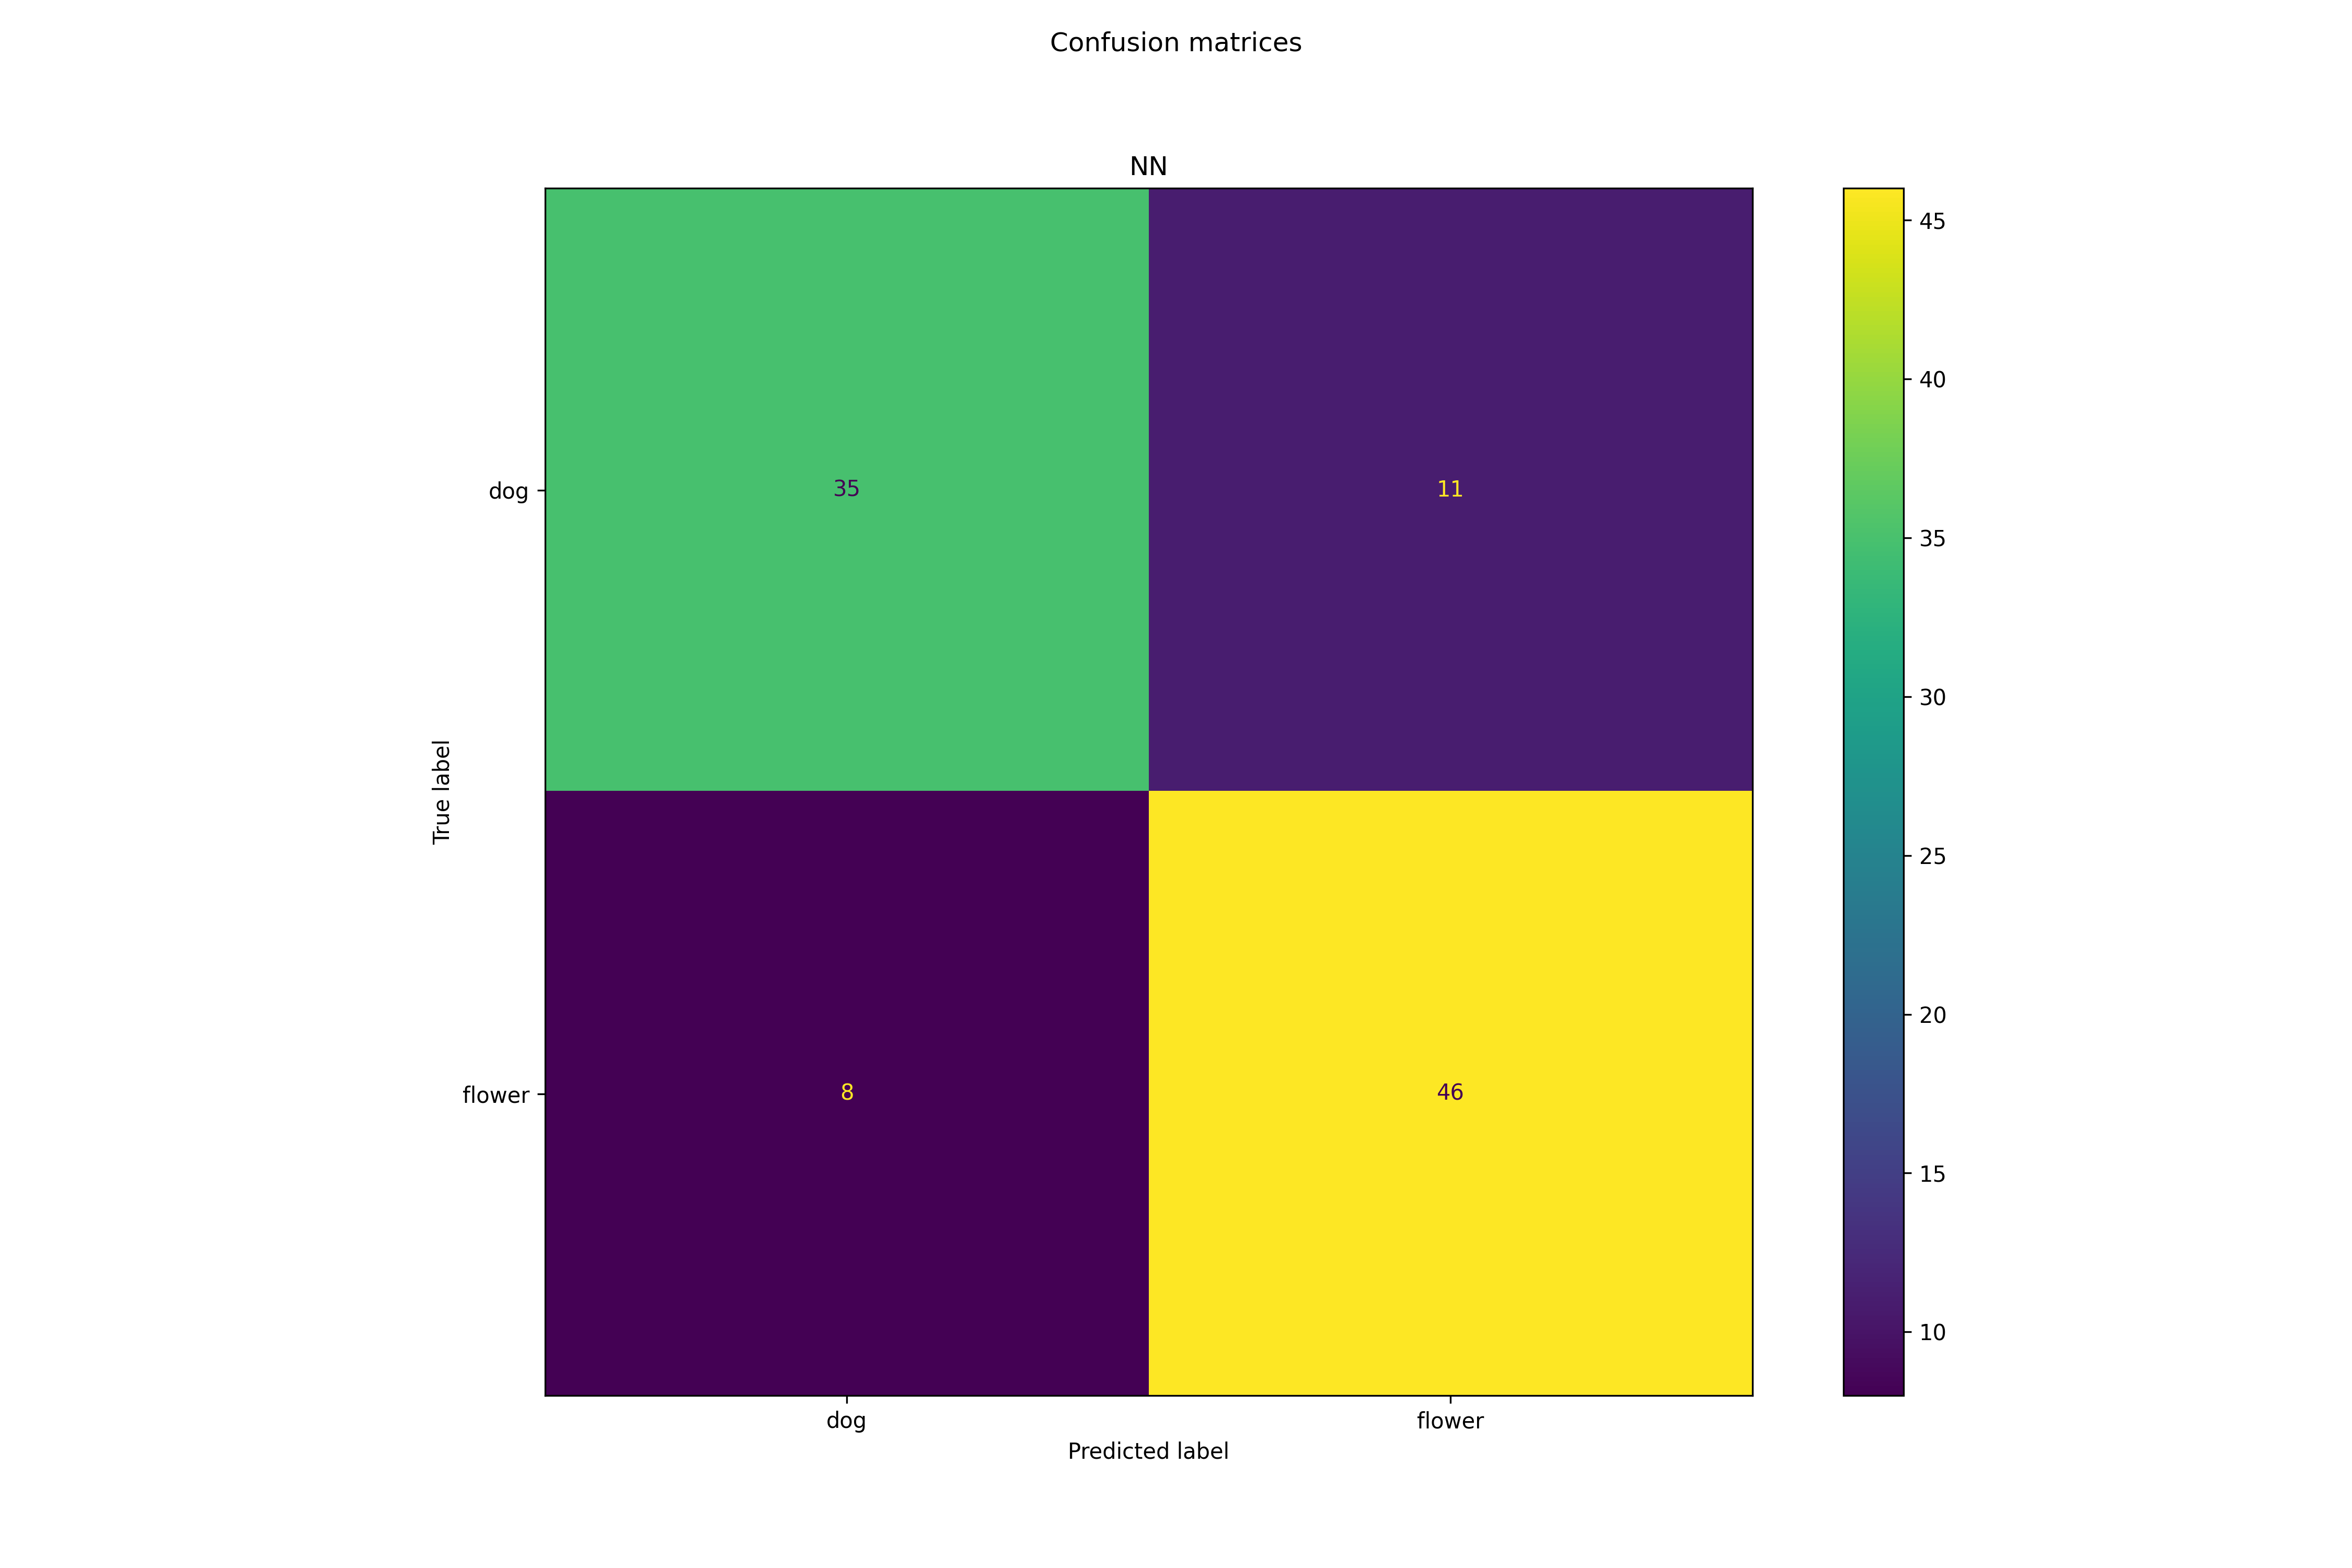
\includegraphics[width=1.3\textwidth]{2.senza_augmentationNN/conf_mat.png}
    \caption{Confusion matrix}
    \label{fig:image-set4-sub1}
  \end{subfigure}
  \hspace{-0.5cm}
  \begin{subfigure}[t]{0.49\textwidth}
    \centering
    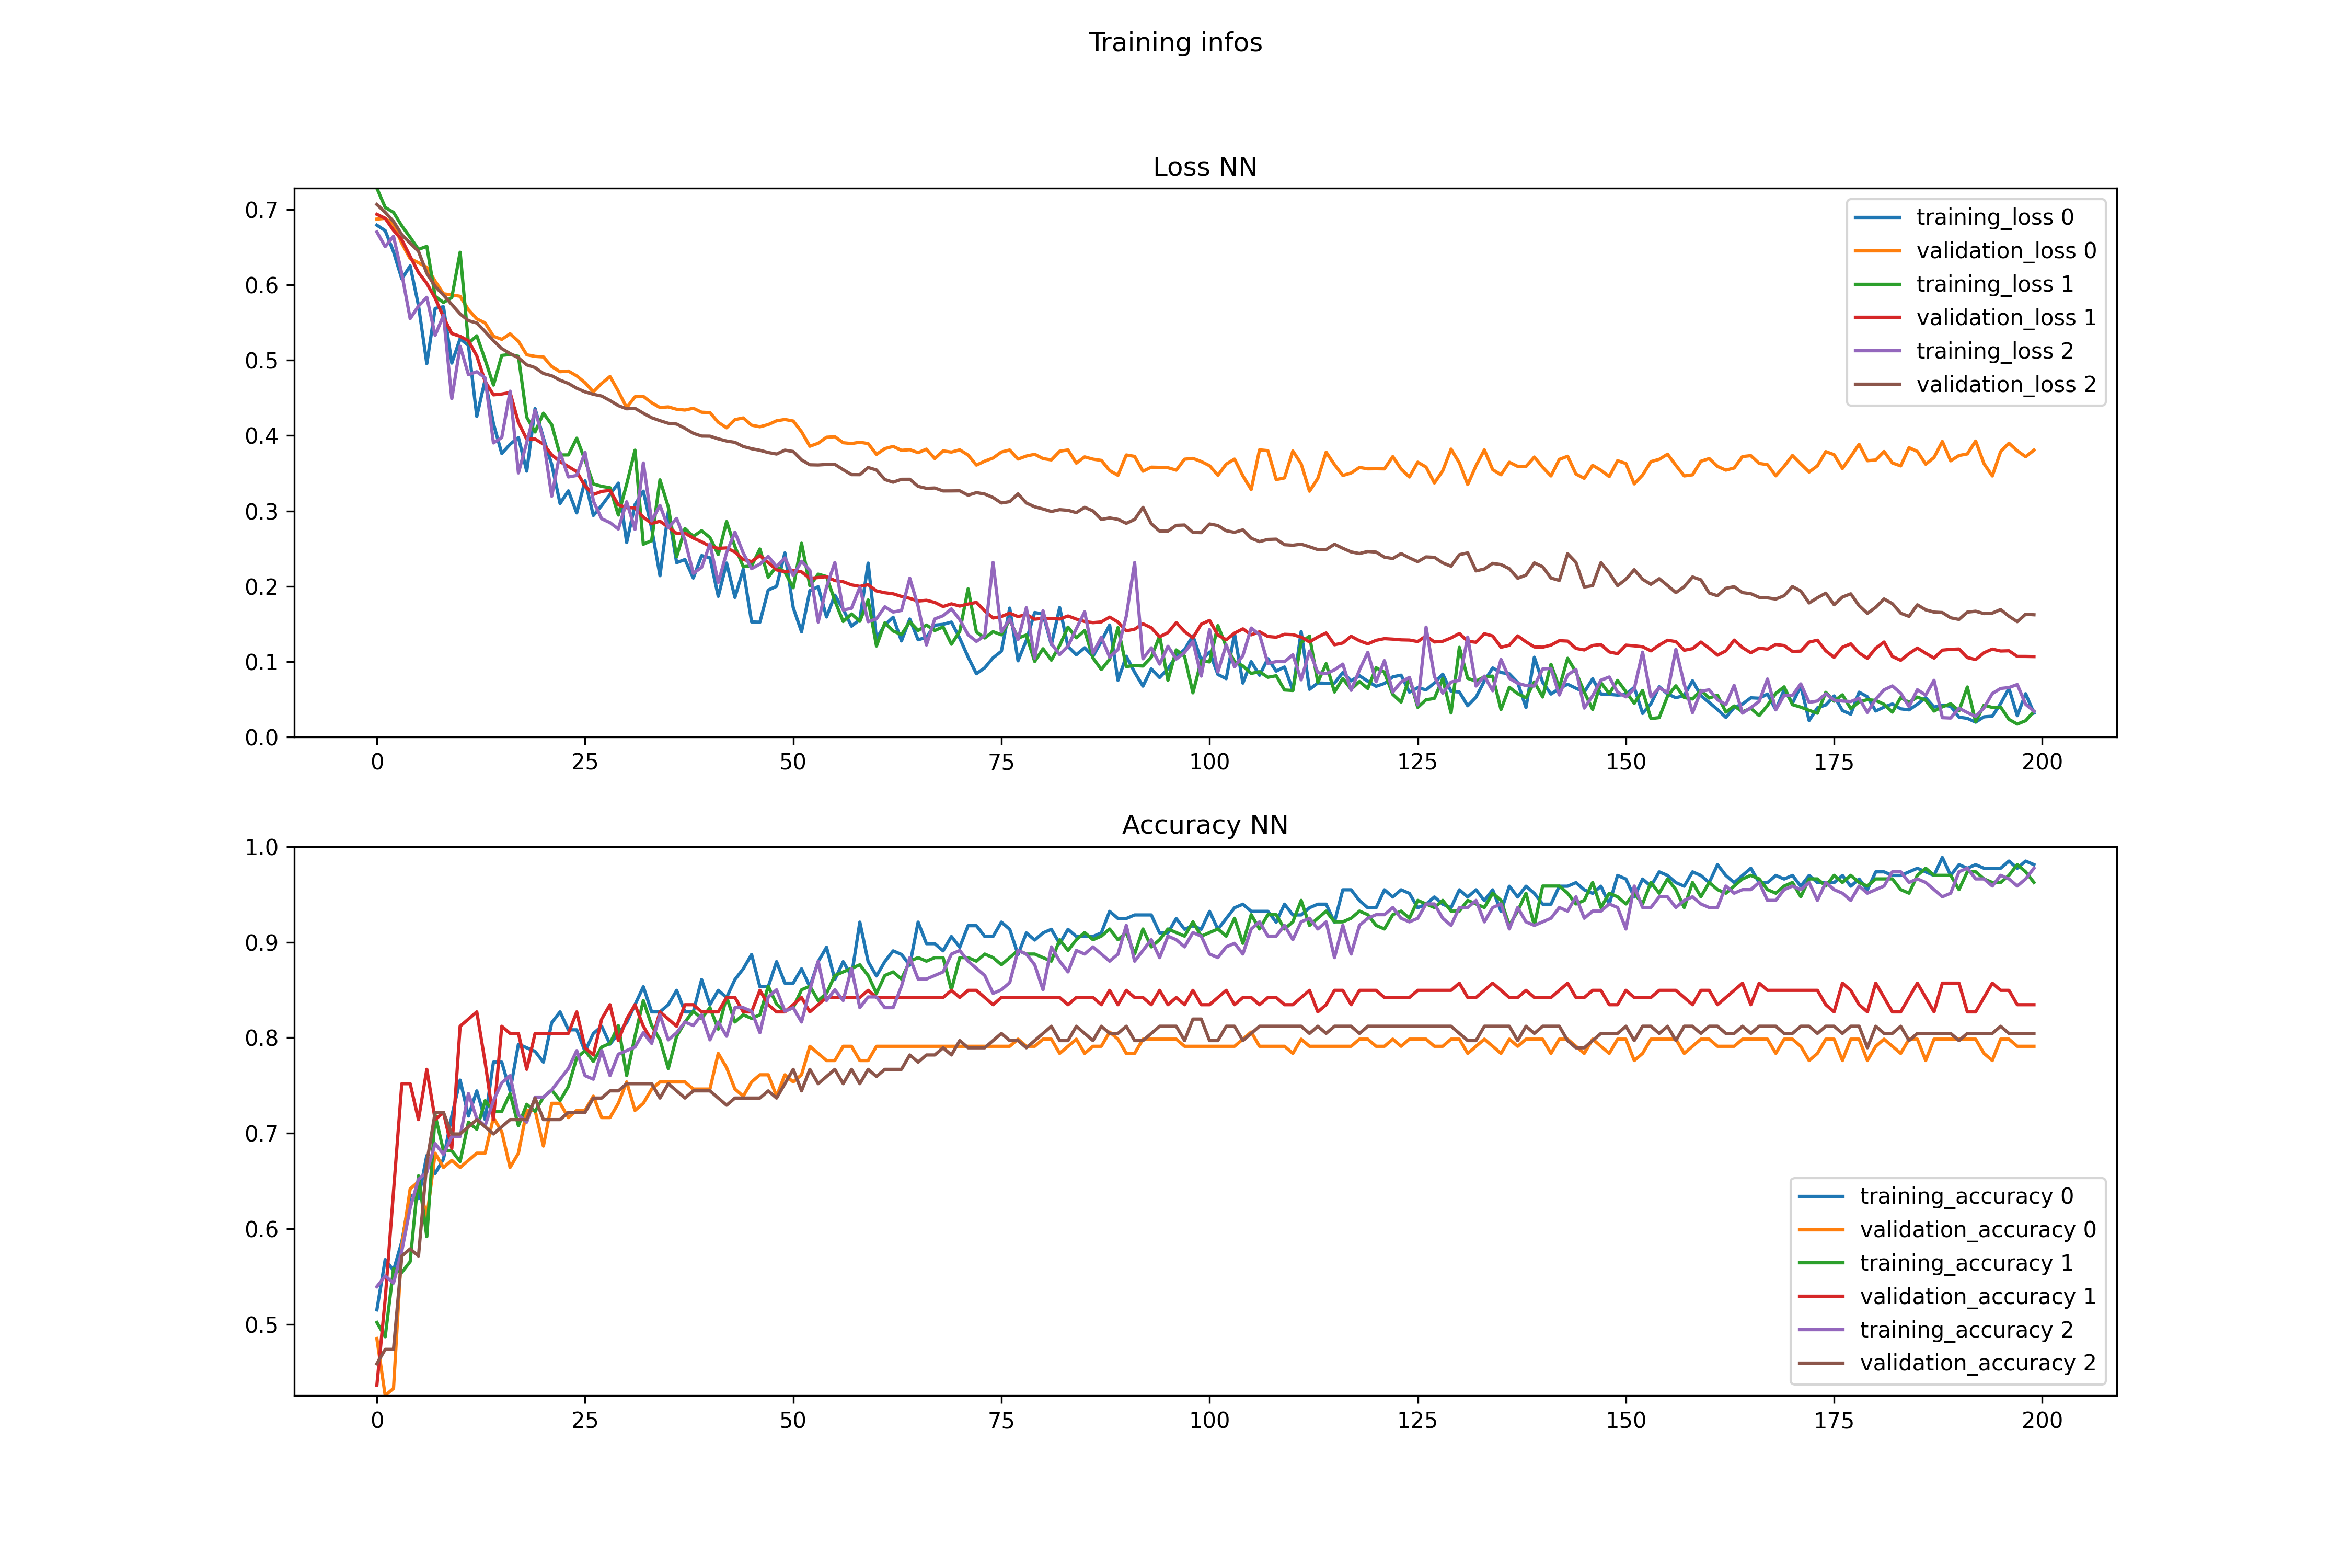
\includegraphics[width=1.3\textwidth]{2.senza_augmentationNN/training_infos.png}
    \caption{Loss and Validation graphs}
    \label{fig:image-set4-sub2}
  \end{subfigure}

  \caption{NN executions without agumentation. The \textbf{accuracy} reached in test is $0.81$.}
  \label{fig:image-set4}
\end{figure}

\begin{figure}[t!]
  \centering
  \hspace{-2cm}
  \begin{subfigure}[t]{0.49\textwidth}
    \centering
    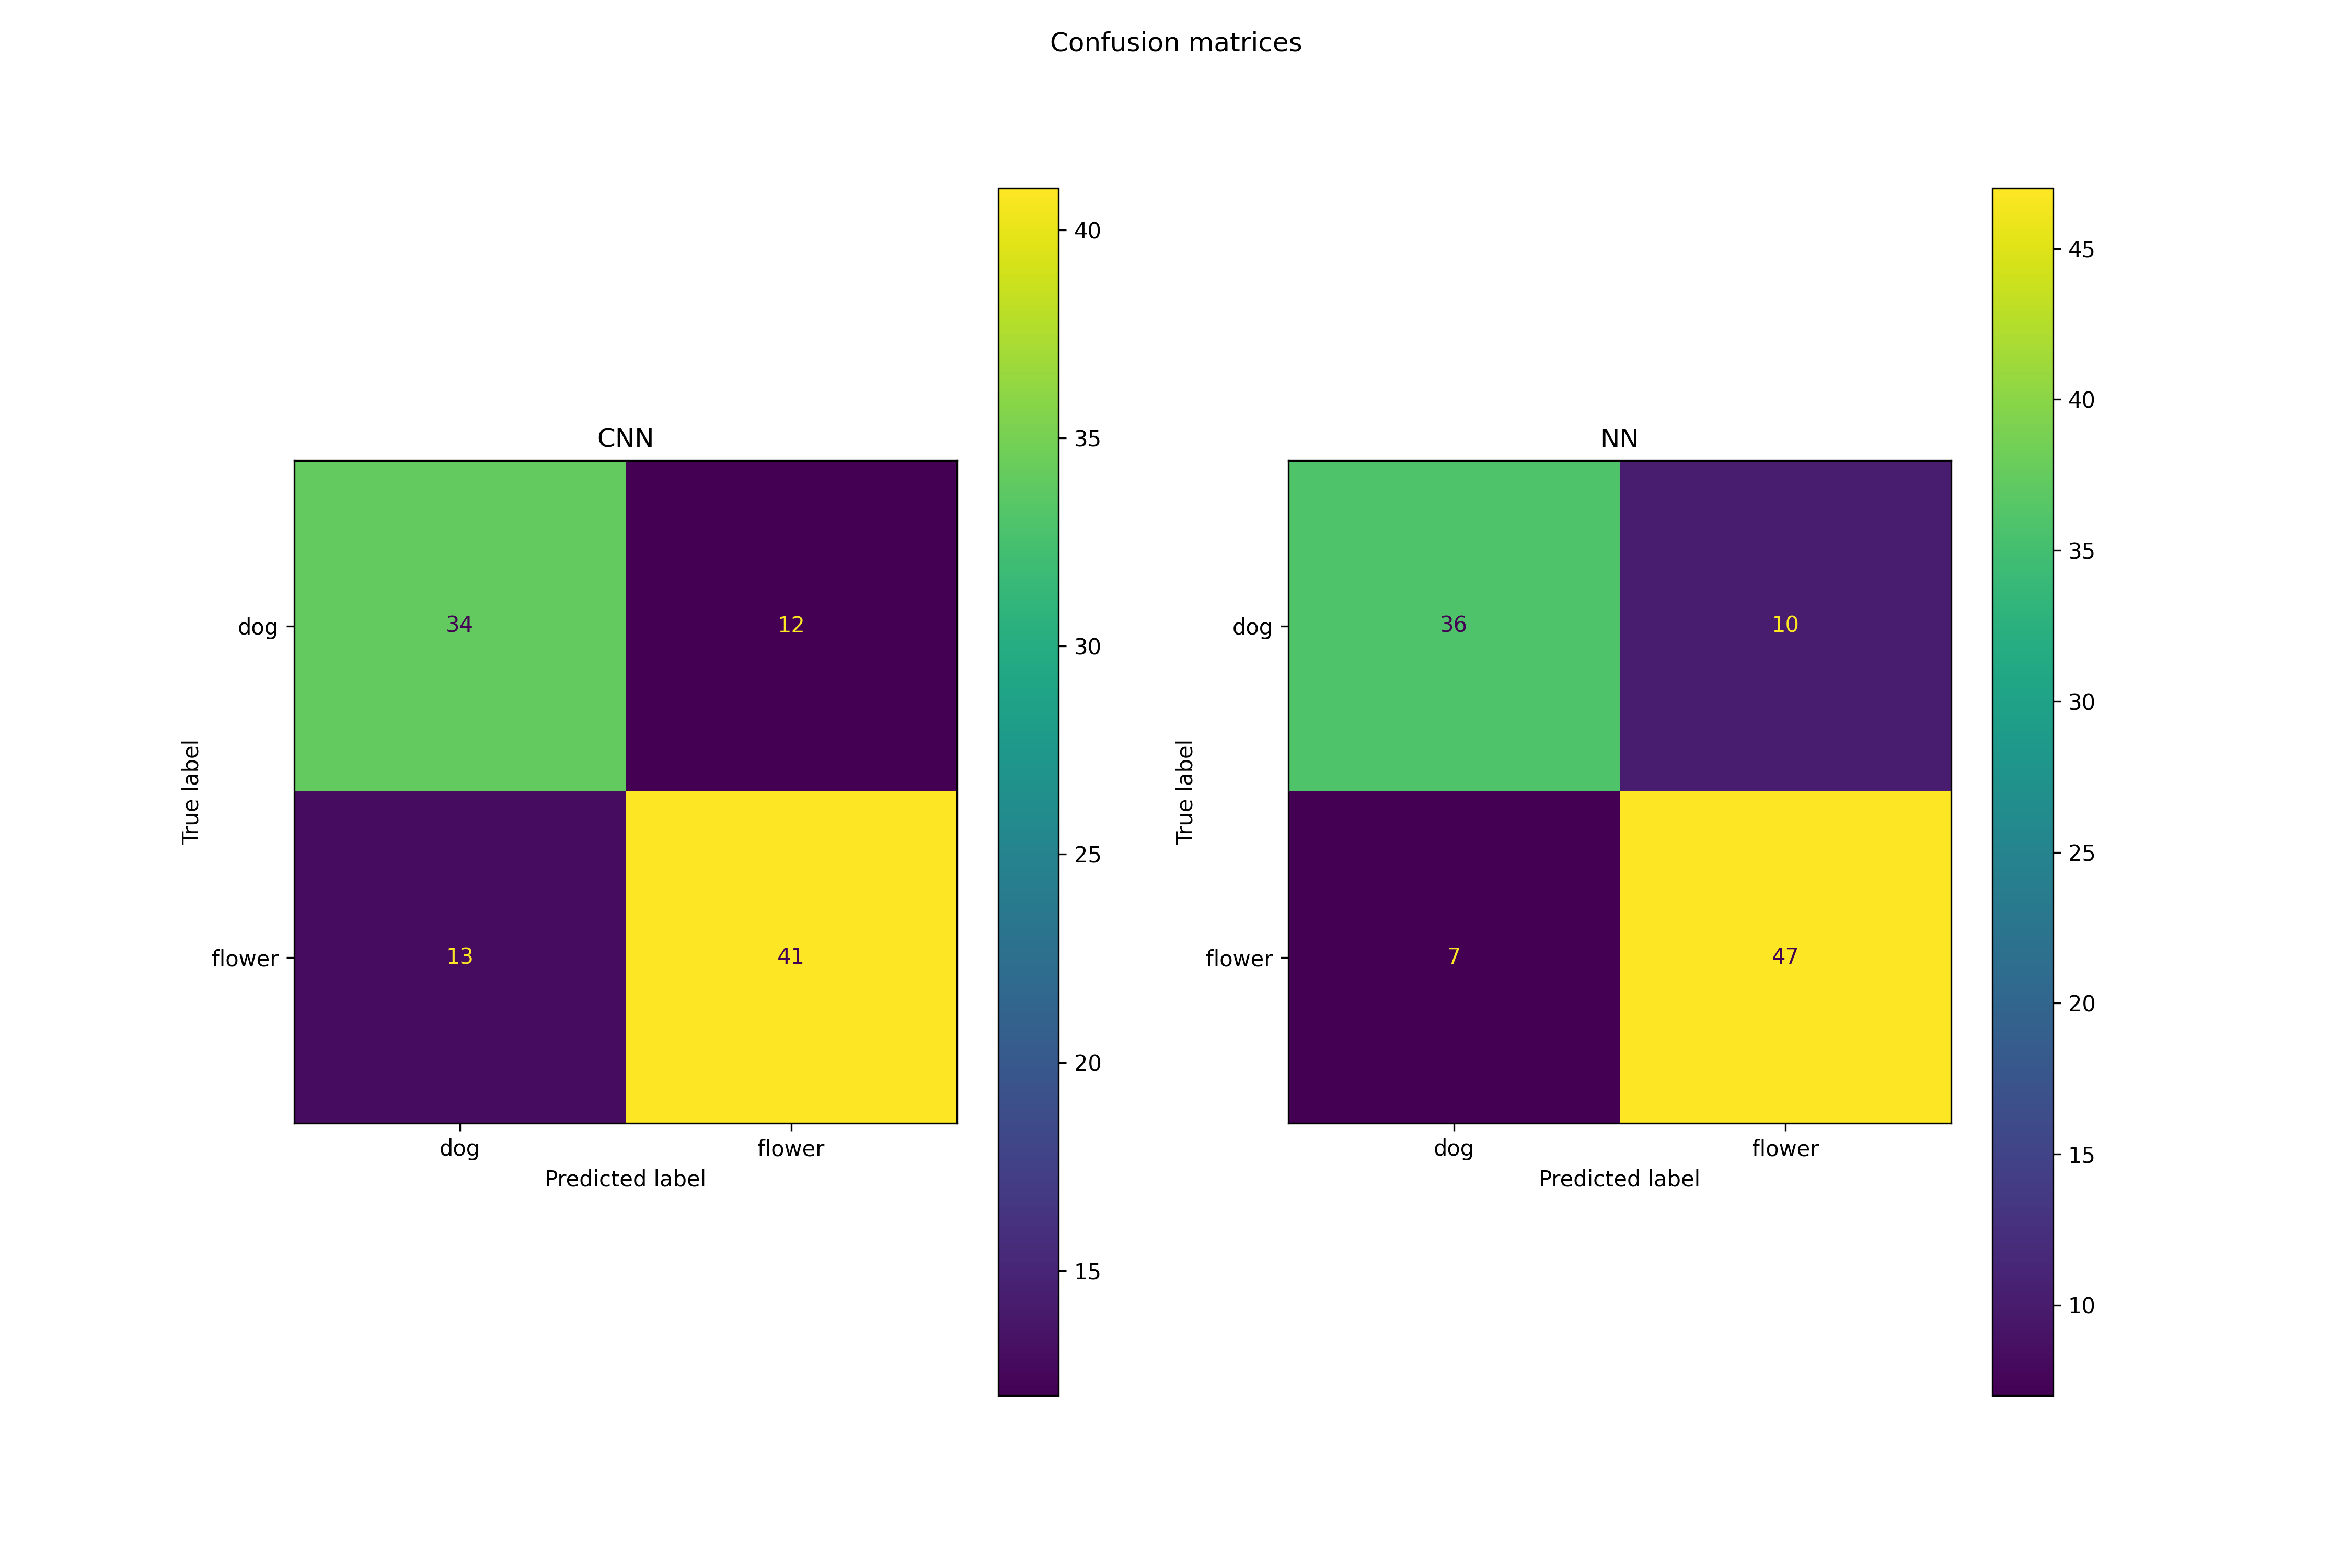
\includegraphics[width=1.3\textwidth]{8.500_noaug/conf_mat.png}
    \caption{Confusion matrix comparison}
    \label{fig:image-set5-sub1}
  \end{subfigure}
  \hfill
  \begin{subfigure}[t]{0.49\textwidth}
    \centering
    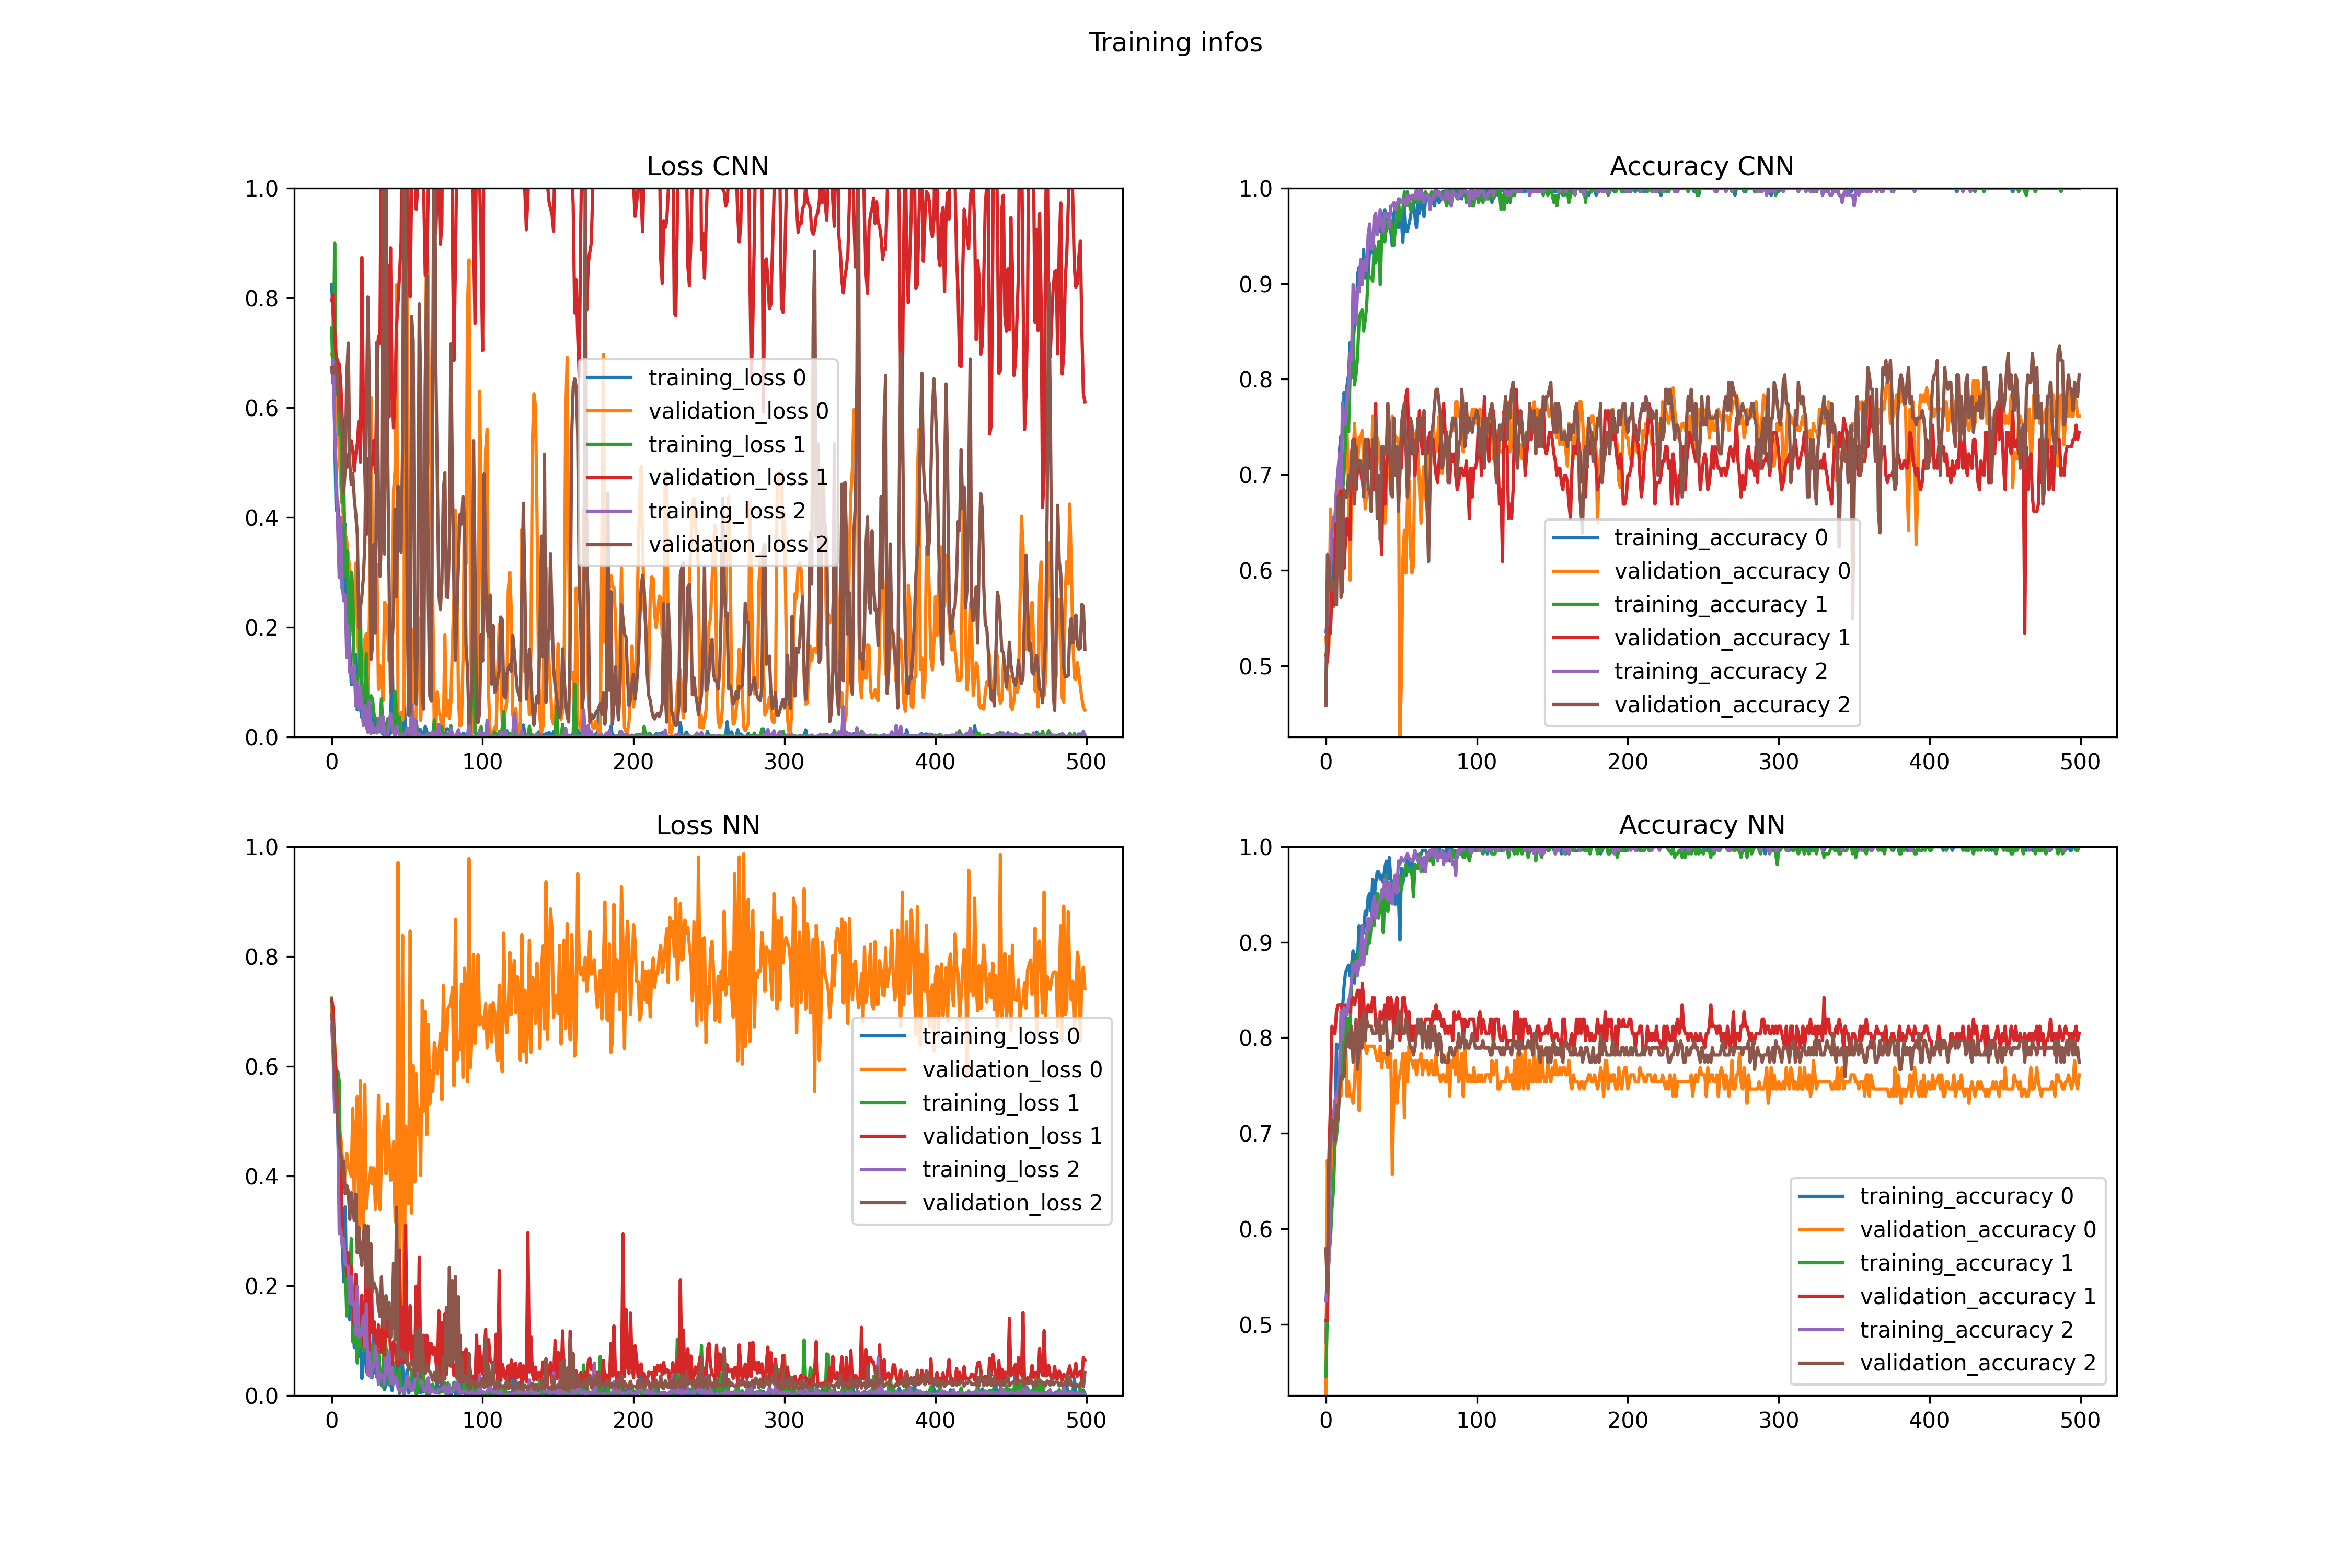
\includegraphics[width=1.3\textwidth]{8.500_noaug/training_infos.png}
    \caption{Traning graphs comparison}
    \label{fig:image-set5-sub2}
  \end{subfigure}

  \caption{Execution with 500 samples and no augmentation. The NN reaches a better accuracy with 83\%, while the CNN reaches 75\%. No augmentation privileges scatter+NN}
  \label{fig:image-set5}
\end{figure}

\begin{figure}[t!]
  \centering
  \hspace{-2cm}
  \begin{subfigure}[t]{0.49\textwidth}
    \centering
    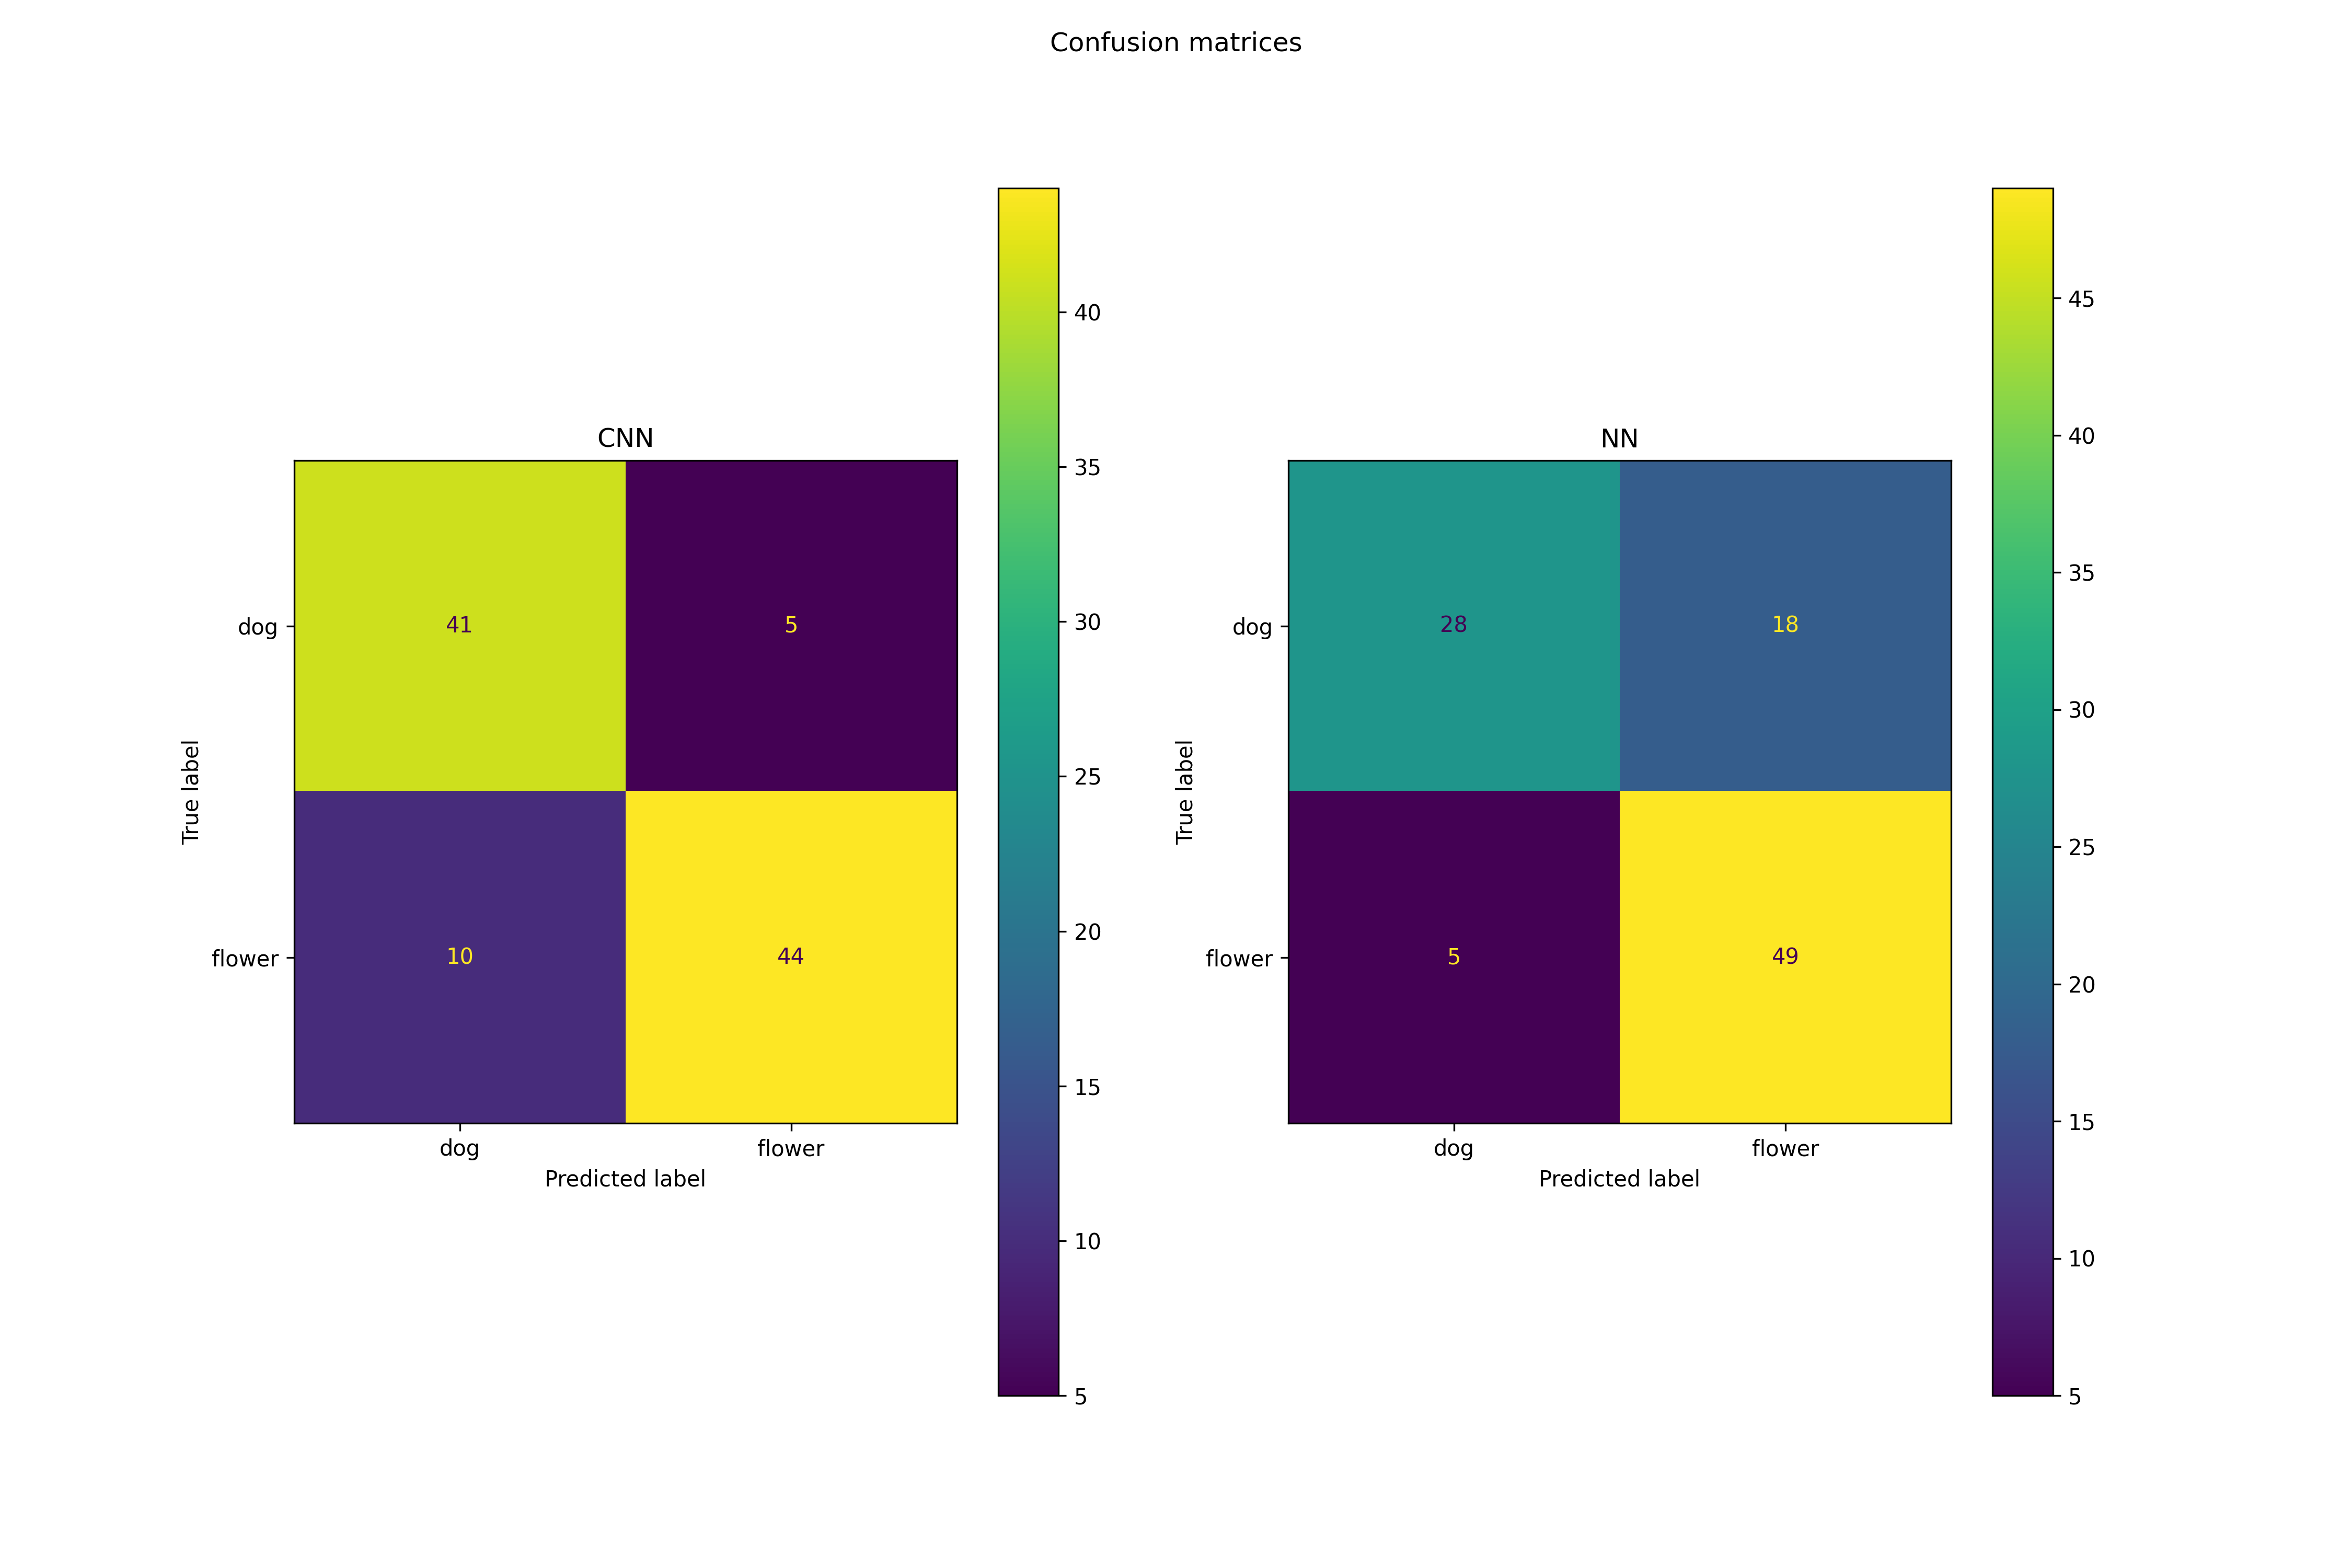
\includegraphics[width=1.3\textwidth]{10.500_aug16/conf_mat.png}
    \caption{Confusion matrix comparison}
    \label{fig:image-set6-sub1}
  \end{subfigure}
  \hfill
  \begin{subfigure}[t]{0.49\textwidth}
    \centering
    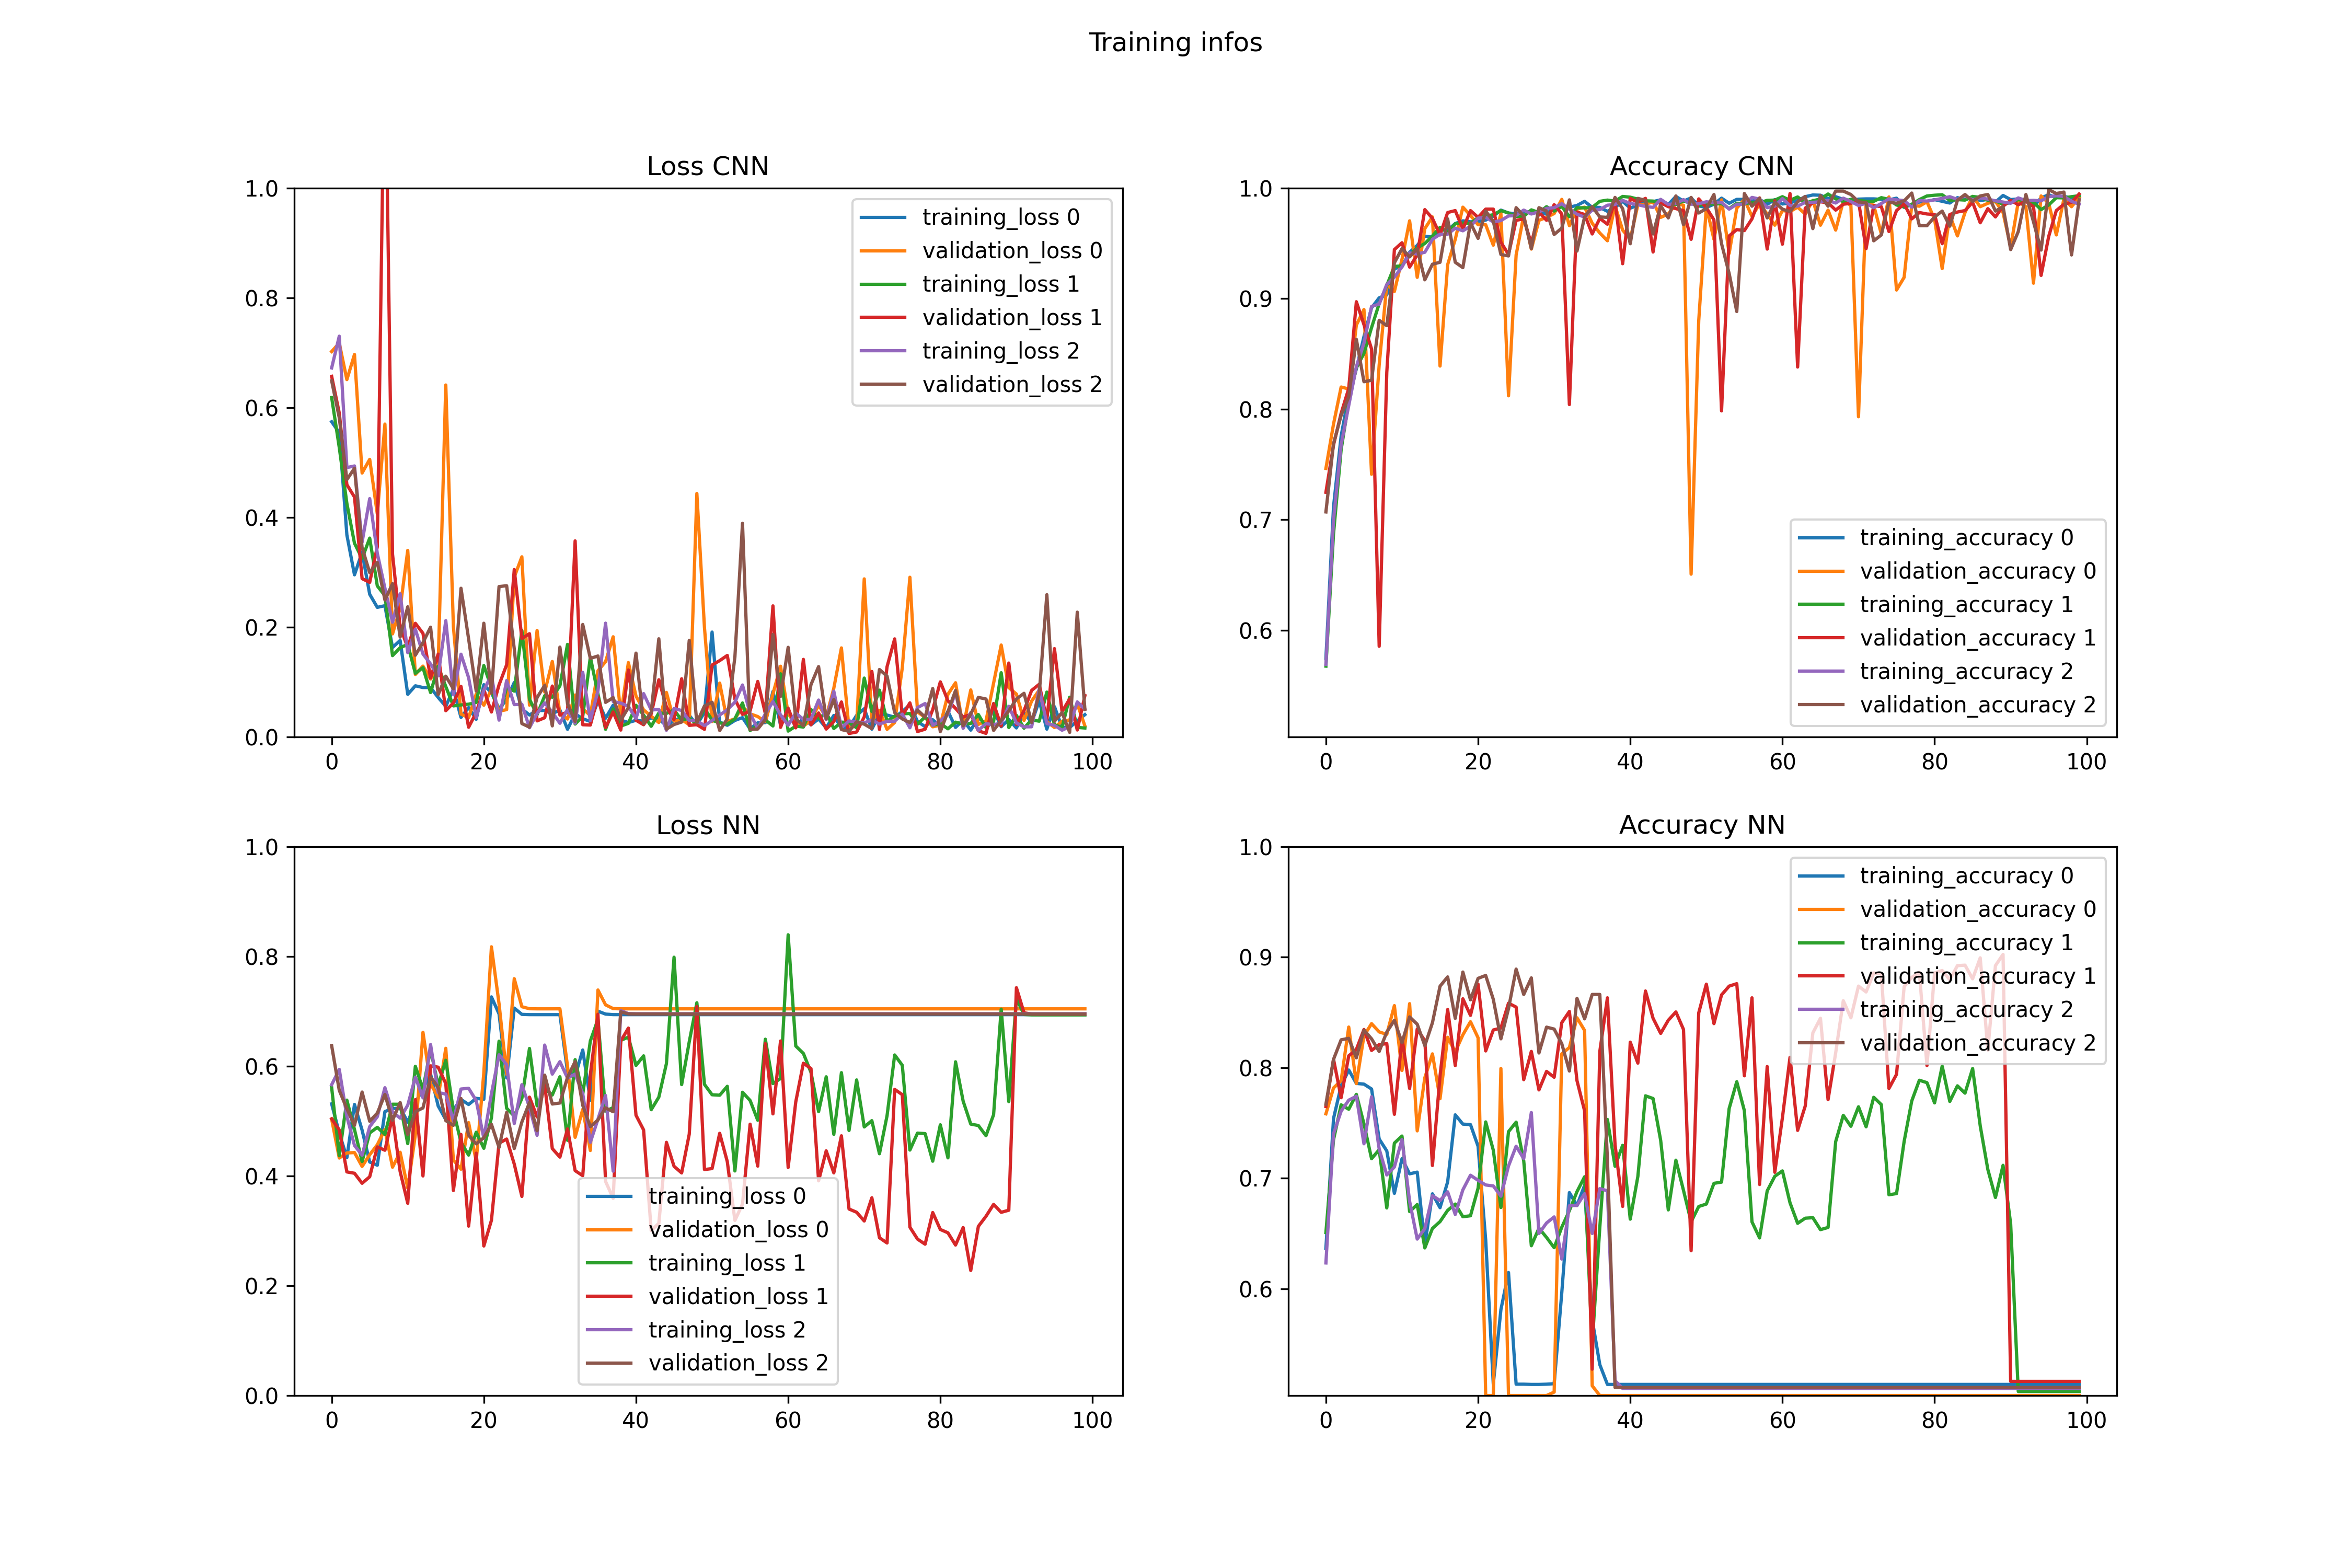
\includegraphics[width=1.3\textwidth]{10.500_aug16/training_infos.png}
    \caption{Traning graphs comparison}
    \label{fig:image-set6-sub2}
  \end{subfigure}

  \caption{Execution with 500 samples and 16 augmentations. The CNN reaches a better accuracy with 0.85\%, while the NN reaches 0.77\%. Augmentation privileges CNN}
  \label{fig:image-set6}
\end{figure}


\end{document}